
%%%%%%%%%%%%%%%%%%%%%%%%%%%%%%%%%%%%%%%%%%%%%%%%%%%%%%%%%%%%%%%%%%%%%%%%%%%%%%%%
%% ************************************************************************** %%
%% *                                Settings                                * %%
%% ************************************************************************** %%
%%%%%%%%%%%%%%%%%%%%%%%%%%%%%%%%%%%%%%%%%%%%%%%%%%%%%%%%%%%%%%%%%%%%%%%%%%%%%%%%
\documentclass{tron}

\loadglsentries{gls}
\glsaddall
\addbibresource{reference}
\usepackage{xcolor}  % Coloured text etc.
% fancy note style
% STYLE NOTES : v2.0
% additional fancy boxes
\usepackage[framemethod=TikZ]{mdframed}
%\usepackage{amsthm}

% gray color indicates [OPTIONAL READING]

%%%%%%%%%%%%%%%%%%%%%%%%%%%%%%
%Note
\newenvironment{note}[3][]{%
	\ifstrempty{#1}%
	{\mdfsetup{%
	frametitle={%
	\tikz[baseline=(current bounding box.east),outer sep=0pt]
	\node[anchor=east,rectangle,fill=#2]
	{\strut Note};}}
	}%
	{\mdfsetup{%
	frametitle={%
	\tikz[baseline=(current bounding box.east),outer sep=0pt]
	\node[anchor=east,rectangle,fill=#2]
	{\strut #1};}}%
	}%
	\mdfsetup{innertopmargin=0pt,skipabove=5pt,linecolor=#2,%
		linewidth=2pt,topline=true,%
		frametitleaboveskip=\dimexpr-\ht\strutbox\relax,
		backgroundcolor={white!90!#2}}
	\begin{mdframed}[]\relax%
	\label{#3}}{\end{mdframed}
}
\Crefname{note}{Note}{notes}

\newcommand{\createnoteenv}[6]{
	\refstepcounter{#6}%
	\ifstrempty{#1}%
	{\mdfsetup{%
	frametitle={%
	\tikz[baseline=(current bounding box.east),outer sep=0pt]
	\node[anchor=east,rectangle,fill=#3]
	{\strut #4~#5};}}
	}%
	{
		\mdfsetup{%
			frametitle={%
				\tikz[baseline=(current bounding box.east),outer sep=0pt]
				\node[anchor=east,rectangle,fill=#3]
				{\strut #4~#5:~#1};
			}
		}%
	}%
	\mdfsetup{innertopmargin=0pt,skipabove=5pt,linecolor=#3,%
	linewidth=2pt,topline=true,%
	frametitleaboveskip=\dimexpr-\ht\strutbox\relax,
	backgroundcolor={white!90!#3}}
	\begin{mdframed}[]\relax%
	\label{#2}
}

%%%%%%%%%%%%%%%%%%%%%%%%%%%%%%
%Definition
\newcounter{definition}[section] \setcounter{definition}{0}
\renewcommand{\thedefinition}{\arabic{section}.\arabic{definition}}
\newenvironment{definition}[2][]{%
	\createnoteenv{#1}{#2}{blue!40}{Definition}{\thedefinition}{definition}%
}{\end{mdframed}}
\newenvironment{definition*}[2][]{%
	\createnoteenv{#1}{#2}{gray!40}{Definition}{\thedefinition}{definition}%
}{\end{mdframed}}
\Crefname{definition}{Definition}{definitions}


%%%%%%%%%%%%%%%%%%%%%%%%%%%%%%
%theoremrem
\newcounter{theorem}[section] \setcounter{theorem}{0}
\renewcommand{\thetheorem}{\arabic{section}.\arabic{theorem}}
\newenvironment{theorem}[2][]{%
	\createnoteenv{#1}{#2}{cyan!40}{Theorem}{\thetheorem}{theorem}%
}{\end{mdframed}}
\newenvironment{theorem*}[2][]{%
	\createnoteenv{#1}{#2}{gray!40}{Theorem}{\thetheorem}{theorem}%
}{\end{mdframed}}
\Crefname{theorem}{Theorem}{theorems}

%%%%%%%%%%%%%%%%%%%%%%%%%%%%%%
%Proof
\newcounter{proof}[section]\setcounter{proof}{0}
\renewcommand{\theproof}{\arabic{section}.\arabic{proof}}
\newenvironment{proof}[2][]{%
	\createnoteenv{#1}{#2}{red!20}{Proof}{\theproof}{proof}%
}{\end{mdframed}}
\newenvironment{proof*}[2][]{%
	\createnoteenv{#1}{#2}{gray!40}{Proof}{\theproof}{proof}%
}{\end{mdframed}}
\Crefname{proof}{Proof}{proofs}


%%%%%%%%%%%%%%%%%%%%%%%%%%%%%%
%Alert
\newcounter{alert}[section]\setcounter{alert}{0}
\renewcommand{\thealert}{\arabic{section}.\arabic{alert}}
\newenvironment{alert}[2][]{%
	\createnoteenv{#1}{#2}{red!80}{Alert}{\thealert}{alert}%
}{\end{mdframed}}
\newenvironment{alert*}[2][]{%
	\createnoteenv{#1}{#2}{gray!40}{Alert}{\thealert}{alert}%
}{\end{mdframed}}
\Crefname{alert}{Alert}{alerts}

%%%%%%%%%%%%%%%%%%%%%%%%%%%%%%
%Answer
\newcounter{answer}[section]\setcounter{answer}{0}
\renewcommand{\theanswer}{\arabic{section}.\arabic{answer}}
\newenvironment{answer}[2][]{%
	\createnoteenv{#1}{#2}{orange!60}{Answer}{\theanswer}{answer}%
}{\end{mdframed}}
\newenvironment{answer*}[2][]{%
	\createnoteenv{#1}{#2}{gray!40}{Answer}{\theanswer}{answer}%
}{\end{mdframed}}
\Crefname{answer}{Answer}{answers}

%%%%%%%%%%%%%%%%%%%%%%%%%%%%%%
%Remark
\newcounter{remark}[section]\setcounter{remark}{0}
\renewcommand{\theremark}{\arabic{section}.\arabic{remark}}
\newenvironment{remark}[2][]{%
	\createnoteenv{#1}{#2}{orange!40}{Remark}{\theremark}{remark}%
}{\end{mdframed}}
\newenvironment{remark*}[2][]{%
	\createnoteenv{#1}{#2}{gray!40}{Remark}{\theremark}{remark}%
}{\end{mdframed}}
\Crefname{remark}{Remark}{remarks}


%%%%%%%%%%%%%%%%%%%%%%%%%%%%%%%
%%Example
%\newcounter{example}[section]\setcounter{example}{0}
%\renewcommand{\theexample}{\arabic{section}.\arabic{example}}
%\newenvironment{example}[2][]{%
%	\createnoteenv{#1}{#2}{blue!40!cyan!20}{Example}{\theexample}{example}%
%}{\end{mdframed}}
%\newenvironment{example*}[2][]{%
%	\createnoteenv{#1}{#2}{gray!40}{Example}{\theexample}{example}%
%}{\end{mdframed}}

%%%%%%%%%%%%%%%%%%%%%%%%%%%%%%
%Algorithm
\newcounter{algo}[section]\setcounter{algo}{0}
\renewcommand{\thealgo}{\arabic{algo}.\arabic{algo}}
\newenvironment{algo}[2][]{%
	\createnoteenv{#1}{#2}{yellow!90!brown!60}{Algorithm}{\thealgo}{algo}%
}{\end{mdframed}}
\newenvironment{algo*}[2][]{%
	\createnoteenv{#1}{#2}{gray!40}{Algorithm}{\thealgo}{algo}%
}{\end{mdframed}}
\Crefname{algo}{Algorithm}{algos}

%%%%%%%%%%%%%%%%%%%%%%%%%%%%%%
% CS480 - Exercise
%\setlength{\parskip}{1cm}
%\setlength{\parindent}{1cm}

%\tikzstyle{titregris} =
%[draw=gray,fill=white, shading = exersicetitle, %
%text=gray, rectangle, rounded corners, right,minimum height=.3cm]
%\pgfdeclarehorizontalshading{exersicebackground}{100bp}
%{color(0bp)=(green!40); color(100bp)=(black!5)}
%\pgfdeclarehorizontalshading{exersicetitle}{100bp}
%{color(0bp)=(red!40);color(100bp)=(black!5)}
%\newcounter{exercise}
%\renewcommand*\theexercise{exercice \textbf{Exercice}~n\arabic{exercise}}
%\makeatletter
%\def\mdf@@exercisepoints{}%new mdframed key:
%\define@key{mdf}{exercisepoints}{%
%\def\mdf@@exercisepoints{#1}
%}
%
%\mdfdefinestyle{theoremstyle}{%
%outerlinewidth=0.01em,linecolor=black,middlelinewidth=0.5pt,%
%frametitlerule=true,roundcorner=2pt,%
%apptotikzsetting={\tikzset{mfframetitlebackground/.append style={%
%shade,left color=white, right color=blue!20}}},
%frametitlerulecolor=black,innertopmargin=1\baselineskip,%green!60,
%innerbottommargin=0.5\baselineskip,
%frametitlerulewidth=0.1pt,
%innertopmargin=0.7\topskip,skipabove={\dimexpr0.2\baselineskip+0.1\topskip\relax},
%frametitleaboveskip=1pt,
%frametitlebelowskip=1pt
%}
%\mdtheorem[style=theoremstyle]{exercise}{\textbf{Exercise}}

\newcounter{exercise}[section]\setcounter{exercise}{0}
\renewcommand{\theexercise}{\arabic{exercise}}
\newenvironment{exercise}[2][]{%
	\createnoteenv{#1}{#2}{gray!40}{Exercise}{\theexercise}{exercise}%
}{\end{mdframed}}
\newenvironment{exercise*}[2][]{%
	\createnoteenv{#1}{#2}{gray!40}{Exercise}{\theexercise}{exercise}%
}{\end{mdframed}}

\Crefname{exercise}{Exercise}{exercises}


%%%%%%%%%%%%%%%%%%%%%%%%%%%%%%
%Examples
% {

%     \section{Theorem and lemma examples with title}
%     \begin{theorem}[Pythagoras' theorem]{theorem:pythagoras}
%     In a right triangle, the square of the hypotenuse is equal to the sum of the squares of the catheti.
%     \[a^2+b^2=c^2\]
%     \end{theorem}
%     In mathematics, the Pythagorean theorem, also known as Pythagoras' theorem (see theorem \ref{theorem:pythagoras}), is a relation in Euclidean geometry among the three sides of a right triangle.
%     
%     \begin{definition}[B\'ezout's identity]{def:bezout}
%     Let $a$ and $b$ be nonzero integers and let $d$ be their greatest common divisor. Then there exist integers $x$ and $y$ such that:
%     \[ax+by=d\]
%     \end{definition}
%     This is a reference to Bezout's lemma \ref{def:bezout}
%     
%     
%     \section{Theorem and proof examples without title}
%     
%     \begin{theorem}[]{theorem:theorem1}
%     There exist two irrational numbers $x$, $y$ such that $x^y$ is rational.
%     \end{theorem}
%     
%     \begin{proof}[]{proof:proof1}
%     If $x=y=\sqrt{2}$ is an example, then we are done; otherwise $\sqrt{2}^{\sqrt{2}}$ is irrational, in which case taking $x=\sqrt{2}^{\sqrt{2}}$ and $y=\sqrt{2}$ gives us:
%     \[\bigg(\sqrt{2}^{\sqrt{2}}\bigg)^{\sqrt{2}}=\sqrt{2}^{\sqrt{2}\sqrt{2}}=\sqrt{2}^{2}=2.\]
%     \end{proof}
%
%     \begin{alert}[]{alert:alert1}
%     If $x=y=\sqrt{2}$ is an example, then we are done; otherwise $\sqrt{2}^{\sqrt{2}}$ is irrational, in which case taking $x=\sqrt{2}^{\sqrt{2}}$ and $y=\sqrt{2}$ gives us:
%     \[\bigg(\sqrt{2}^{\sqrt{2}}\bigg)^{\sqrt{2}}=\sqrt{2}^{\sqrt{2}\sqrt{2}}=\sqrt{2}^{2}=2.\]
%     \end{alert}
%     
%     \begin{remark}[]{alert:alert1}
%     If $x=y=\sqrt{2}$ is an example, then we are done; otherwise $\sqrt{2}^{\sqrt{2}}$ is irrational, in which case taking $x=\sqrt{2}^{\sqrt{2}}$ and $y=\sqrt{2}$ gives us:
%     \[\bigg(\sqrt{2}^{\sqrt{2}}\bigg)^{\sqrt{2}}=\sqrt{2}^{\sqrt{2}\sqrt{2}}=\sqrt{2}^{2}=2.\]
%     \end{remark}
%     
%     
%          \begin{exercise}[]{alert:alert1}
%     If $x=y=\sqrt{2}$ is an example, then we are done; otherwise $\sqrt{2}^{\sqrt{2}}$ is irrational, in which case taking $x=\sqrt{2}^{\sqrt{2}}$ and $y=\sqrt{2}$ gives us:
%     \[\bigg(\sqrt{2}^{\sqrt{2}}\bigg)^{\sqrt{2}}=\sqrt{2}^{\sqrt{2}\sqrt{2}}=\sqrt{2}^{2}=2.\]
%     \end{exercise}
%     
%     \begin{algo}[]{algorithm:alert1}
%     If $x=y=\sqrt{2}$ is an example, then we are done; otherwise $\sqrt{2}^{\sqrt{2}}$ is irrational, in which case taking $x=\sqrt{2}^{\sqrt{2}}$ and $y=\sqrt{2}$ gives us:
%     \[\bigg(\sqrt{2}^{\sqrt{2}}\bigg)^{\sqrt{2}}=\sqrt{2}^{\sqrt{2}\sqrt{2}}=\sqrt{2}^{2}=2.\]
%     \end{algo}
%     
%     \begin{note}[Goal]{pink}{note:goal}
%     If $x=y=\sqrt{2}$ is an example, then we are done; otherwise $\sqrt{2}^{\sqrt{2}}$ is irrational, in which case taking $x=\sqrt{2}^{\sqrt{2}}$ and $y=\sqrt{2}$ gives us:
%     \[\bigg(\sqrt{2}^{\sqrt{2}}\bigg)^{\sqrt{2}}=\sqrt{2}^{\sqrt{2}\sqrt{2}}=\sqrt{2}^{2}=2.\]
%     \end{note}

% }
%\usepackage{lipsum}                     % Dummytext
\usepackage{xargs}                      % Use more than one optional parameter in a new commands
\usepackage[colorinlistoftodos,prependcaption,textsize=normalsize]{todonotes}
%
\newcommandx{\unsure}[2][1=]{\todo[linecolor=red,backgroundcolor=red!25,bordercolor=red,#1]{#2}}
\newcommandx{\change}[2][1=]{\todo[linecolor=blue,backgroundcolor=blue!25,bordercolor=blue,#1]{#2}}
\newcommandx{\info}[2][1=]{\todo[linecolor=OliveGreen,backgroundcolor=OliveGreen!25,bordercolor=OliveGreen,#1]{#2}}
\newcommandx{\improvement}[2][1=]{\todo[linecolor=Plum,backgroundcolor=Plum!25,bordercolor=Plum,#1]{#2}}
\newcommandx{\thiswillnotshow}[2][1=]{\todo[disable,#1]{#2}}
%
\preto\printlistoftodos{
    \listoftodos[Todo List]
}

% EXAMPLES:
    % \todo[inline]{The original todo note withouth changed colours.\newline Here's another line.}
    % \lipsum[11]\unsure{Is this correct?}\unsure{I'm unsure about also!}
    % \lipsum[11]\change{Change this!}
    % \lipsum[11]\info{This can help me in chapter seven!}
    % \lipsum[11]\improvement{This really needs to be improved!\newline\newline What was I thinking?!}
    % \lipsum[11]
    % \thiswillnotshow{This is hidden since option `disable' is chosen!}
    % \improvement[inline]{The following section needs to be rewritten!}
    % \lipsum[11]
    % \newpage
    % \listoftodos[Notes]
%%%  Equation Condition
\newenvironment{eqconditions}
  {\par\vspace{\abovedisplayskip}\noindent\begin{tabular}{>{$}l<{$} @{${}={}$} l}}
  {\end{tabular}\par\vspace{\belowdisplayskip}}
\newenvironment{eqconditions*}
  {\noindent\begin{tabular}{>{$}l<{$} @{${}={}$} l}}
  {\end{tabular}}
%%% introduce 4th depth with \paragraph command
\usepackage{titlesec}
\setcounter{secnumdepth}{4}
\titleformat{\paragraph}
{\normalfont\normalsize\bfseries}{\theparagraph}{1em}{}
\titlespacing*{\paragraph}
{0pt}{3.25ex plus 1ex minus .2ex}{1.5ex plus .2ex}

%%% enumeration reference
% constraint
\newlist{constraint-list}{enumerate}{1}
\setlist[constraint-list,1]{leftmargin=*, label= \Roman*}
\creflabelformat{Constraint}{#2#1#3}
\crefname{constraint-listi}{Constraint}{position}
% criteria
\newlist{criteria-list}{enumerate}{1}
\setlist[criteria-list,1]{leftmargin=*, label= \Roman*}
\creflabelformat{Criterion}{#2#1#3}
\crefname{criteria-listi}{Criterion}{position}
% property
\newlist{property-list}{enumerate}{1}
\setlist[property-list,1]{leftmargin=*, label= \Roman*}
\creflabelformat{Property}{#2#1#3}
\crefname{property-listi}{Property}{position}
% assumption
\newlist{assumption-list}{enumerate}{1}
\setlist[assumption-list,1]{leftmargin=*, label= \Roman*}
\creflabelformat{Assumption}{#2#1#3}
\crefname{assumption-listi}{Assumption}{position}

% custom math command
\newcommand{\unit}[1]{\left[\si{#1}\right]}

% additional math packages
\usepackage{physics}
\usepackage{cancel}

% TODO Flags
\newcommand\TODO[1]{{\textcolor{red}{\textbf{#1}}}}
\newcommand\COMMENT[1]{\hl{#1}}

% Custom Format
% \usepackage{float}
% \usepackage[table]{xcolor}
% \usepackage{soul}
\usepackage{multirow}
\usepackage{caption} 
\captionsetup[table]{skip=3pt}
\captionsetup[figure]{skip=0pt}
\titlespacing*{\section}
{0pt}{10pt}{3pt}
\titlespacing*{\subsection}
{0pt}{8pt}{3pt}
\titlespacing*{\subsubsection}
{0pt}{8pt}{3pt}
%hide the highlight box
\hypersetup{
    colorlinks,
    linkcolor={black!50!black},
    citecolor={black!50!blue},
    urlcolor={black!80!black}
}%hide the highlight box

% table formatting
% \setlength{\arrayrulewidth}{1mm}
% \setlength{\tabcolsep}{18pt}
% \renewcommand{\arraystretch}{2.5}
\usepackage{array}
\newcolumntype{C}[1]{>{\centering\let\newline\\\arraybackslash\hspace{0pt}}m{#1}}

% custom math symbol
%% CS 480 %%
\newcommand{\bm}[1]{\mathbf{#1}}
%%%%%%%%%%%%
\newcommand{\RR}{\mathds{R}}
\newcommand{\Id}{\mathbb{I}}
\newcommand{\NN}{\mathds{N}}
\newcommand{\sign}{\mathop{\mathrm{sign}}}
\newcommand{\diag}{\mathop{\mathrm{diag}}}
\newcommand{\argmin}{\mathop{\mathrm{argmin}}}
\newcommand{\zero}{\mathbf{0}}
\newcommand{\one}{\mathbf{1}}
\newcommand{\av}{\mathbf{a}}
\newcommand{\bv}{\mathbf{b}}
\newcommand{\sv}{\mathbf{s}}
\newcommand{\Xv}{\mathbf{X}}
\newcommand{\Yv}{\mathbf{Y}}
\newcommand{\wv}{\mathbf{w}}
\newcommand{\xv}{\mathbf{x}}
\newcommand{\yv}{\mathbf{y}}
\newcommand{\zv}{\mathbf{z}}
\newcommand{\uv}{\mathbf{u}}
\newcommand{\rv}{\mathbf{r}}
\newcommand{\inner}[2]{\langle #1, #2 \rangle}
\newcommand{\red}[1]{{\color{red}#1}}
\newcommand{\blue}[1]{{\color{blue}#1}}
\newcommand{\magenta}[1]{{\color{magenta}#1}}


\newcommand{\ea}{{et al.}\xspace}
\newcommand{\eg}{{e.g.}\xspace}
\newcommand{\ie}{{i.e.}\xspace}
\newcommand{\iid}{{i.i.d.}\xspace}
\newcommand{\cf}{{cf.}\xspace}
\newcommand{\wrt}{{w.r.t.}\xspace}
\newcommand{\aka}{{a.k.a.}\xspace}
\newcommand{\etc}{{etc.}\xspace}
\newcommand{\sgm}{\mathsf{sgm}}
\newcommand{\Dc}{\mathcal{D}}
\newcommand{\ans}[1]{{\textcolor{orange}{\textsf{Ans}: #1}}}



% extra mod
\newcommand{\mref}[1]{\underline{\textbf{\hypersetup{linkcolor=orange}\Cref{#1}\hypersetup{linkcolor=blue}}}}
\usepackage{longtable}
\usepackage{float}
\usepackage{color, colortbl}
%%%%%%%%%%%%%%%%%%%%%%%%%%%%%%%%%%%%%%%%%%%%%%%%%%%%%%%%%%%%%%%%%%%%%%%%%%%%%%%%
% Make sure the following block contains the correct information               %
%%%%%%%%%%%%%%%%%%%%%%%%%%%%%%%%%%%%%%%%%%%%%%%%%%%%%%%%%%%%%%%%%%%%%%%%%%%%%%%%
\reporttitle{ECE 457B - Assignment 3}
% \selfstudy % comment this line if this is not a self study report 
% \employername{Employer Name}
% \employerstreetaddress{Employer Address}
% \employerlocation{City, Provice, Country}
\university{University of Waterloo}
\faculty{Faculty of Engineering}%Faculty of Engineering
\department{Department of Electrical and Computer Engineering}%Department of Systems Design Engineering
\groupnumber{1}
\authornameA{Jianxiang (Jack) Xu}
\studentnumberA{20658861}
\reportdate{\today}
%\confidential{1} % comment this line if this is not a confidential report
%\authorstreetaddress{##}
%\authorlocation{##}
%\authorpostalcode{##}
\useheader % comment this line if no need for header
%%%%%%%%%%%%%%%%%%%%%%%%%%%%%%%%%%%%%%%%%%%%%%%%%%%%%%%%%%%%%%%%%%%%%%%%%%%%%%%%
% end of information block...                                                  %
%%%%%%%%%%%%%%%%%%%%%%%%%%%%%%%%%%%%%%%%%%%%%%%%%%%%%%%%%%%%%%%%%%%%%%%%%%%%%%%%

\begin{document}
%%%%%%%%%%%%%%%%%%%%%%%%%%%%%%%%%%%%%%%%%%%%%%%%%%%%%%%%%%%%%%%%%%%%%%%%%%%%%%%%
%% ************************************************************************** %%
%% *                               Title Page                               * %%
%% ************************************************************************** %%
%%%%%%%%%%%%%%%%%%%%%%%%%%%%%%%%%%%%%%%%%%%%%%%%%%%%%%%%%%%%%%%%%%%%%%%%%%%%%%%%
\maketitle
%%%%%%%%%%%%%%%%%%%%%%%%%%%%%%%%%%%%%%%%%%%%%%%%%%%%%%%%%%%%%%%%%%%%%%%%%%%%%%%%
%% ************************************************************************** %%
%% *                           Table of Contents                            * %%
%% ************************************************************************** %%
%%%%%%%%%%%%%%%%%%%%%%%%%%%%%%%%%%%%%%%%%%%%%%%%%%%%%%%%%%%%%%%%%%%%%%%%%%%%%%%%
\tableofcontents
%%%%%%%%%%%%%%%%%%%%%%%%%%%%%%%%%%%%%%%%%%%%%%%%%%%%%%%%%%%%%%%%%%%%%%%%%%%%%%%%
%% ************************************************************************** %%
%% *                            List of Figures                             * %%
%% ************************************************************************** %%
%%%%%%%%%%%%%%%%%%%%%%%%%%%%%%%%%%%%%%%%%%%%%%%%%%%%%%%%%%%%%%%%%%%%%%%%%%%%%%%%
% \listoffigures
%%%%%%%%%%%%%%%%%%%%%%%%%%%%%%%%%%%%%%%%%%%%%%%%%%%%%%%%%%%%%%%%%%%%%%%%%%%%%%%%
%% ************************************************************************** %%
%% *                             List of Tables                             * %%
%% ************************************************************************** %%
%%%%%%%%%%%%%%%%%%%%%%%%%%%%%%%%%%%%%%%%%%%%%%%%%%%%%%%%%%%%%%%%%%%%%%%%%%%%%%%%
% \listoftables
%%%%%%%%%%%%%%%%%%%%%%%%%%%%%%%%%%%%%%%%%%%%%%%%%%%%%%%%%%%%%%%%%%%%%%%%%%%%%%%%
%% ************************************************************************** %%
%% *                              MAIN BODY                                 * %%
%% ************************************************************************** %%
%%%%%%%%%%%%%%%%%%%%%%%%%%%%%%%%%%%%%%%%%%%%%%%%%%%%%%%%%%%%%%
\clearpage
\pagenumbering{arabic}
\setcounter{page}{1}
\setlength{\parskip}{5pt}
\newpage

%%%%%%%%%%%%%%%%%%%%%%%%%%%%%%%%%%%
%%%%% Intro.  %%%%%%
%%%%%%%%%%%%%%%%%%%%%%%%%%%%%%%%%%%

%%%%%%%%%%%%%%%%
%%%%% Ex 1 %%%%%
%%%%%%%%%%%%%%%%
\section{Problem 1 (20 marks): Three Measures of Fuzziness [See Implementation in \Cref{code:p1}]}
\begin{figure}[H]
	\centering
	\subfloat[$M_1$: Closeness to grade 0.5 \label{fig:p1:M1}]{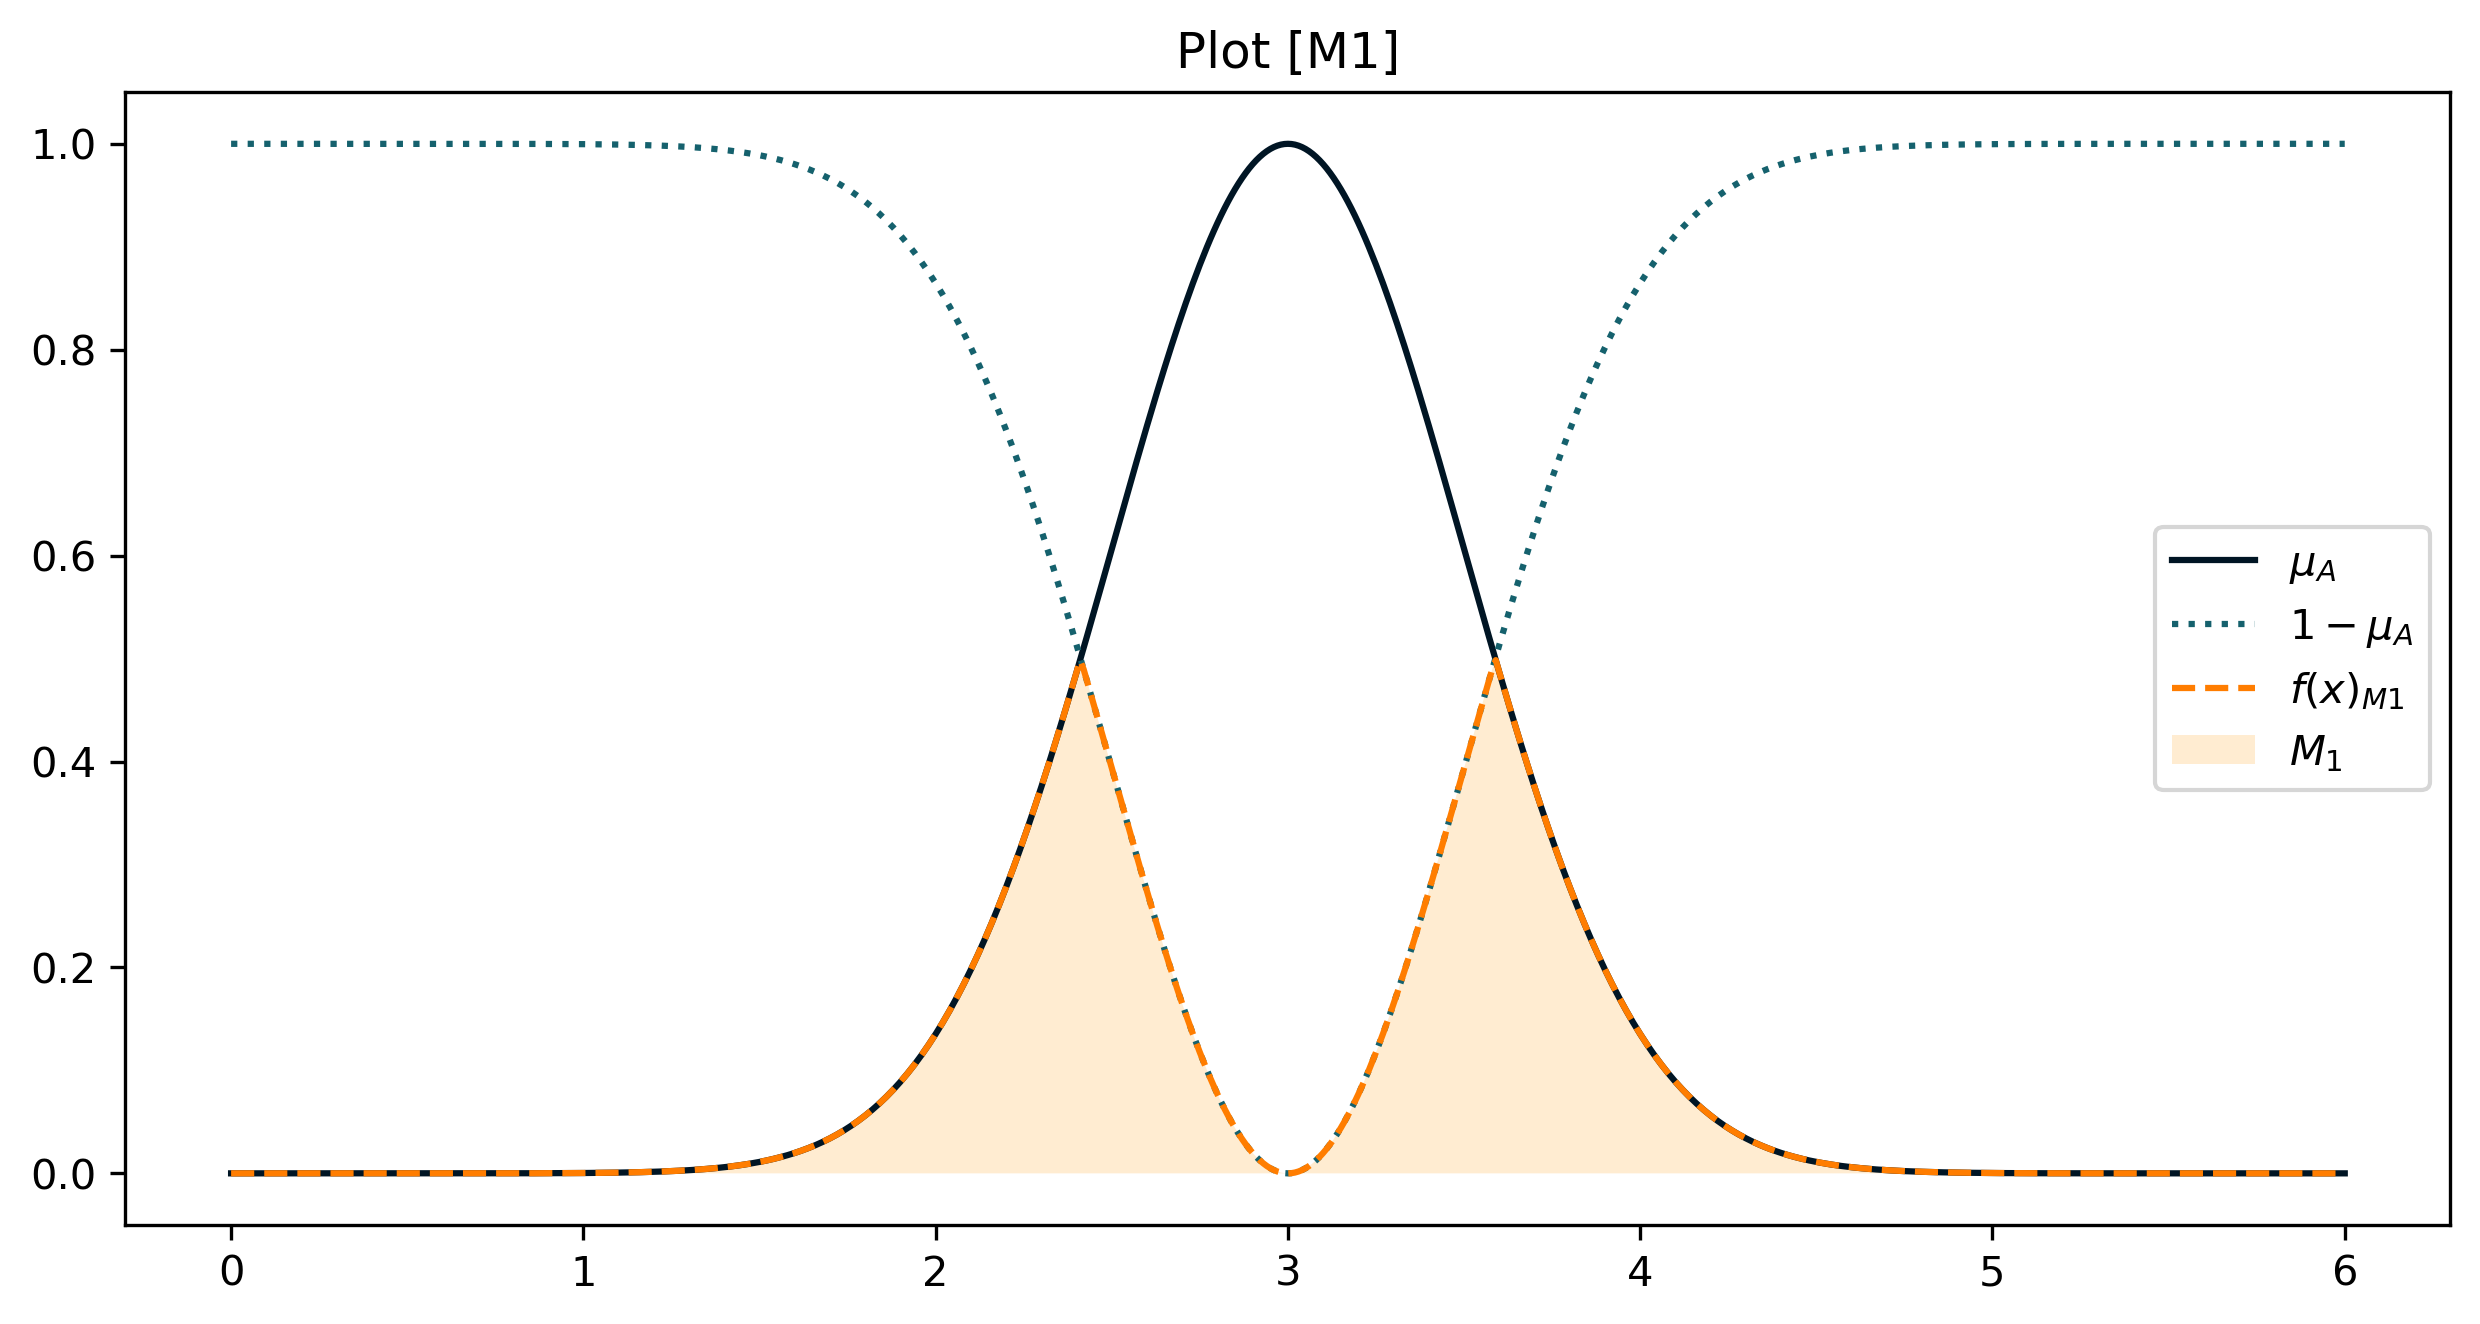
\includegraphics[height=190px]{../src_code/output/P1/plot_M1}} \\
	\subfloat[$M_2$: Distance from 0.5-cut \label{fig:p1:M2}]{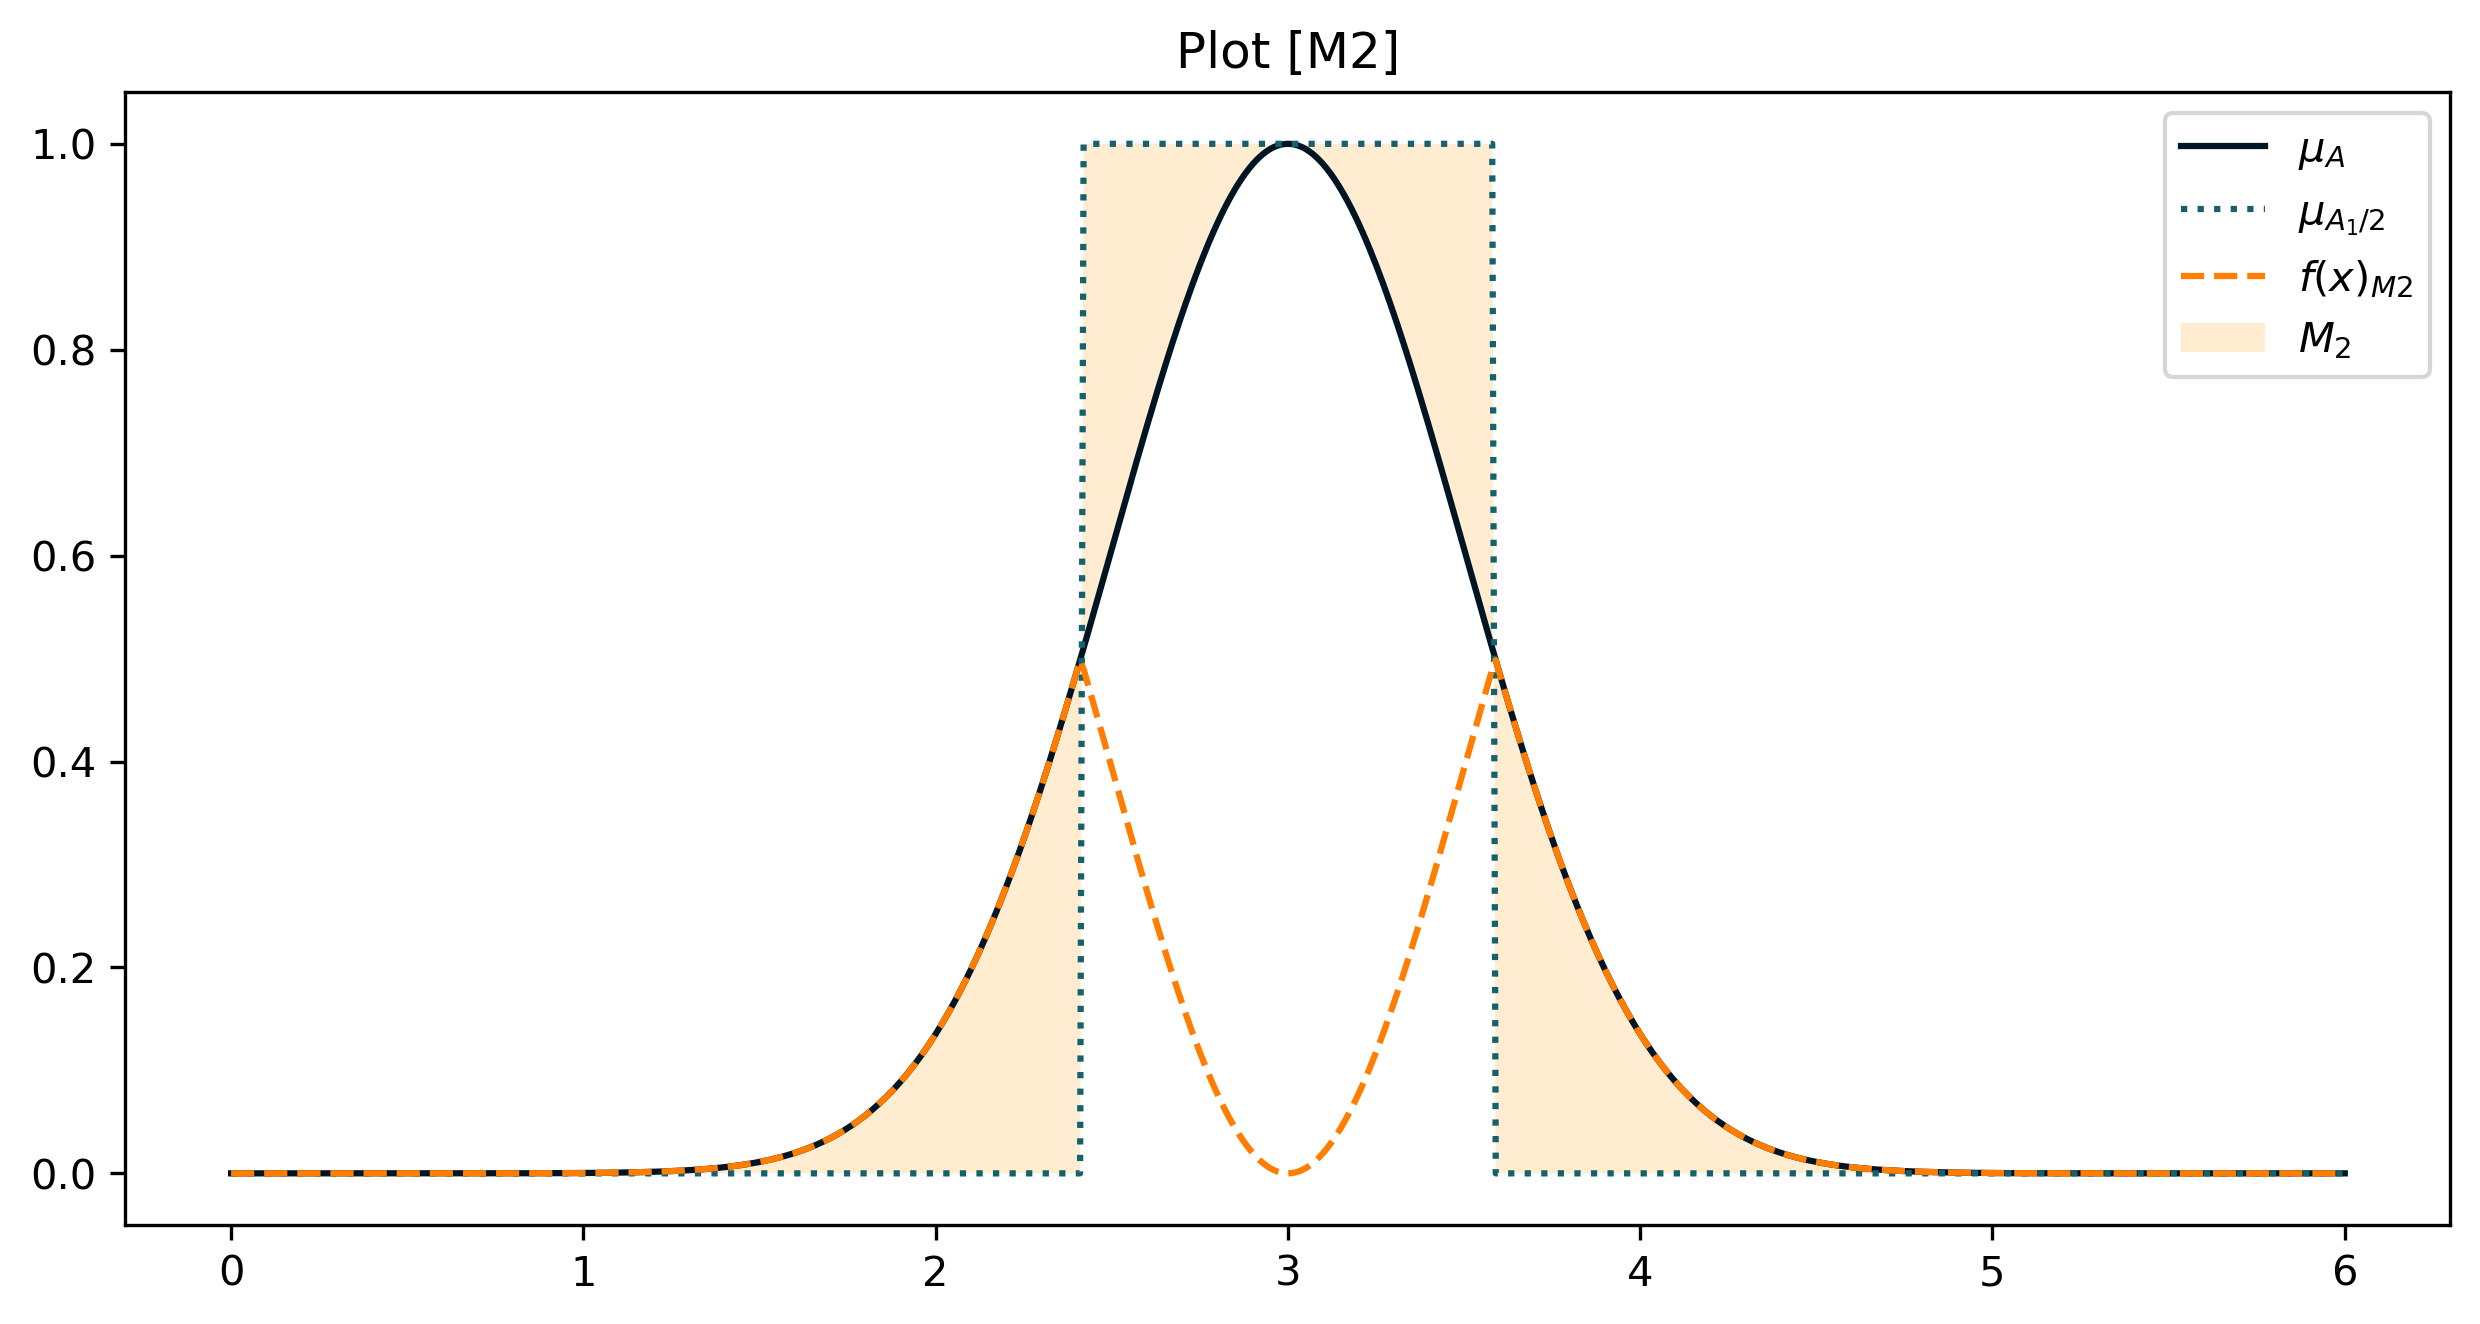
\includegraphics[height=190px]{../src_code/output/P1/plot_M2}} \\
	\subfloat[$M_3$: Inverse of distance from the complement \label{fig:p1:M3}]{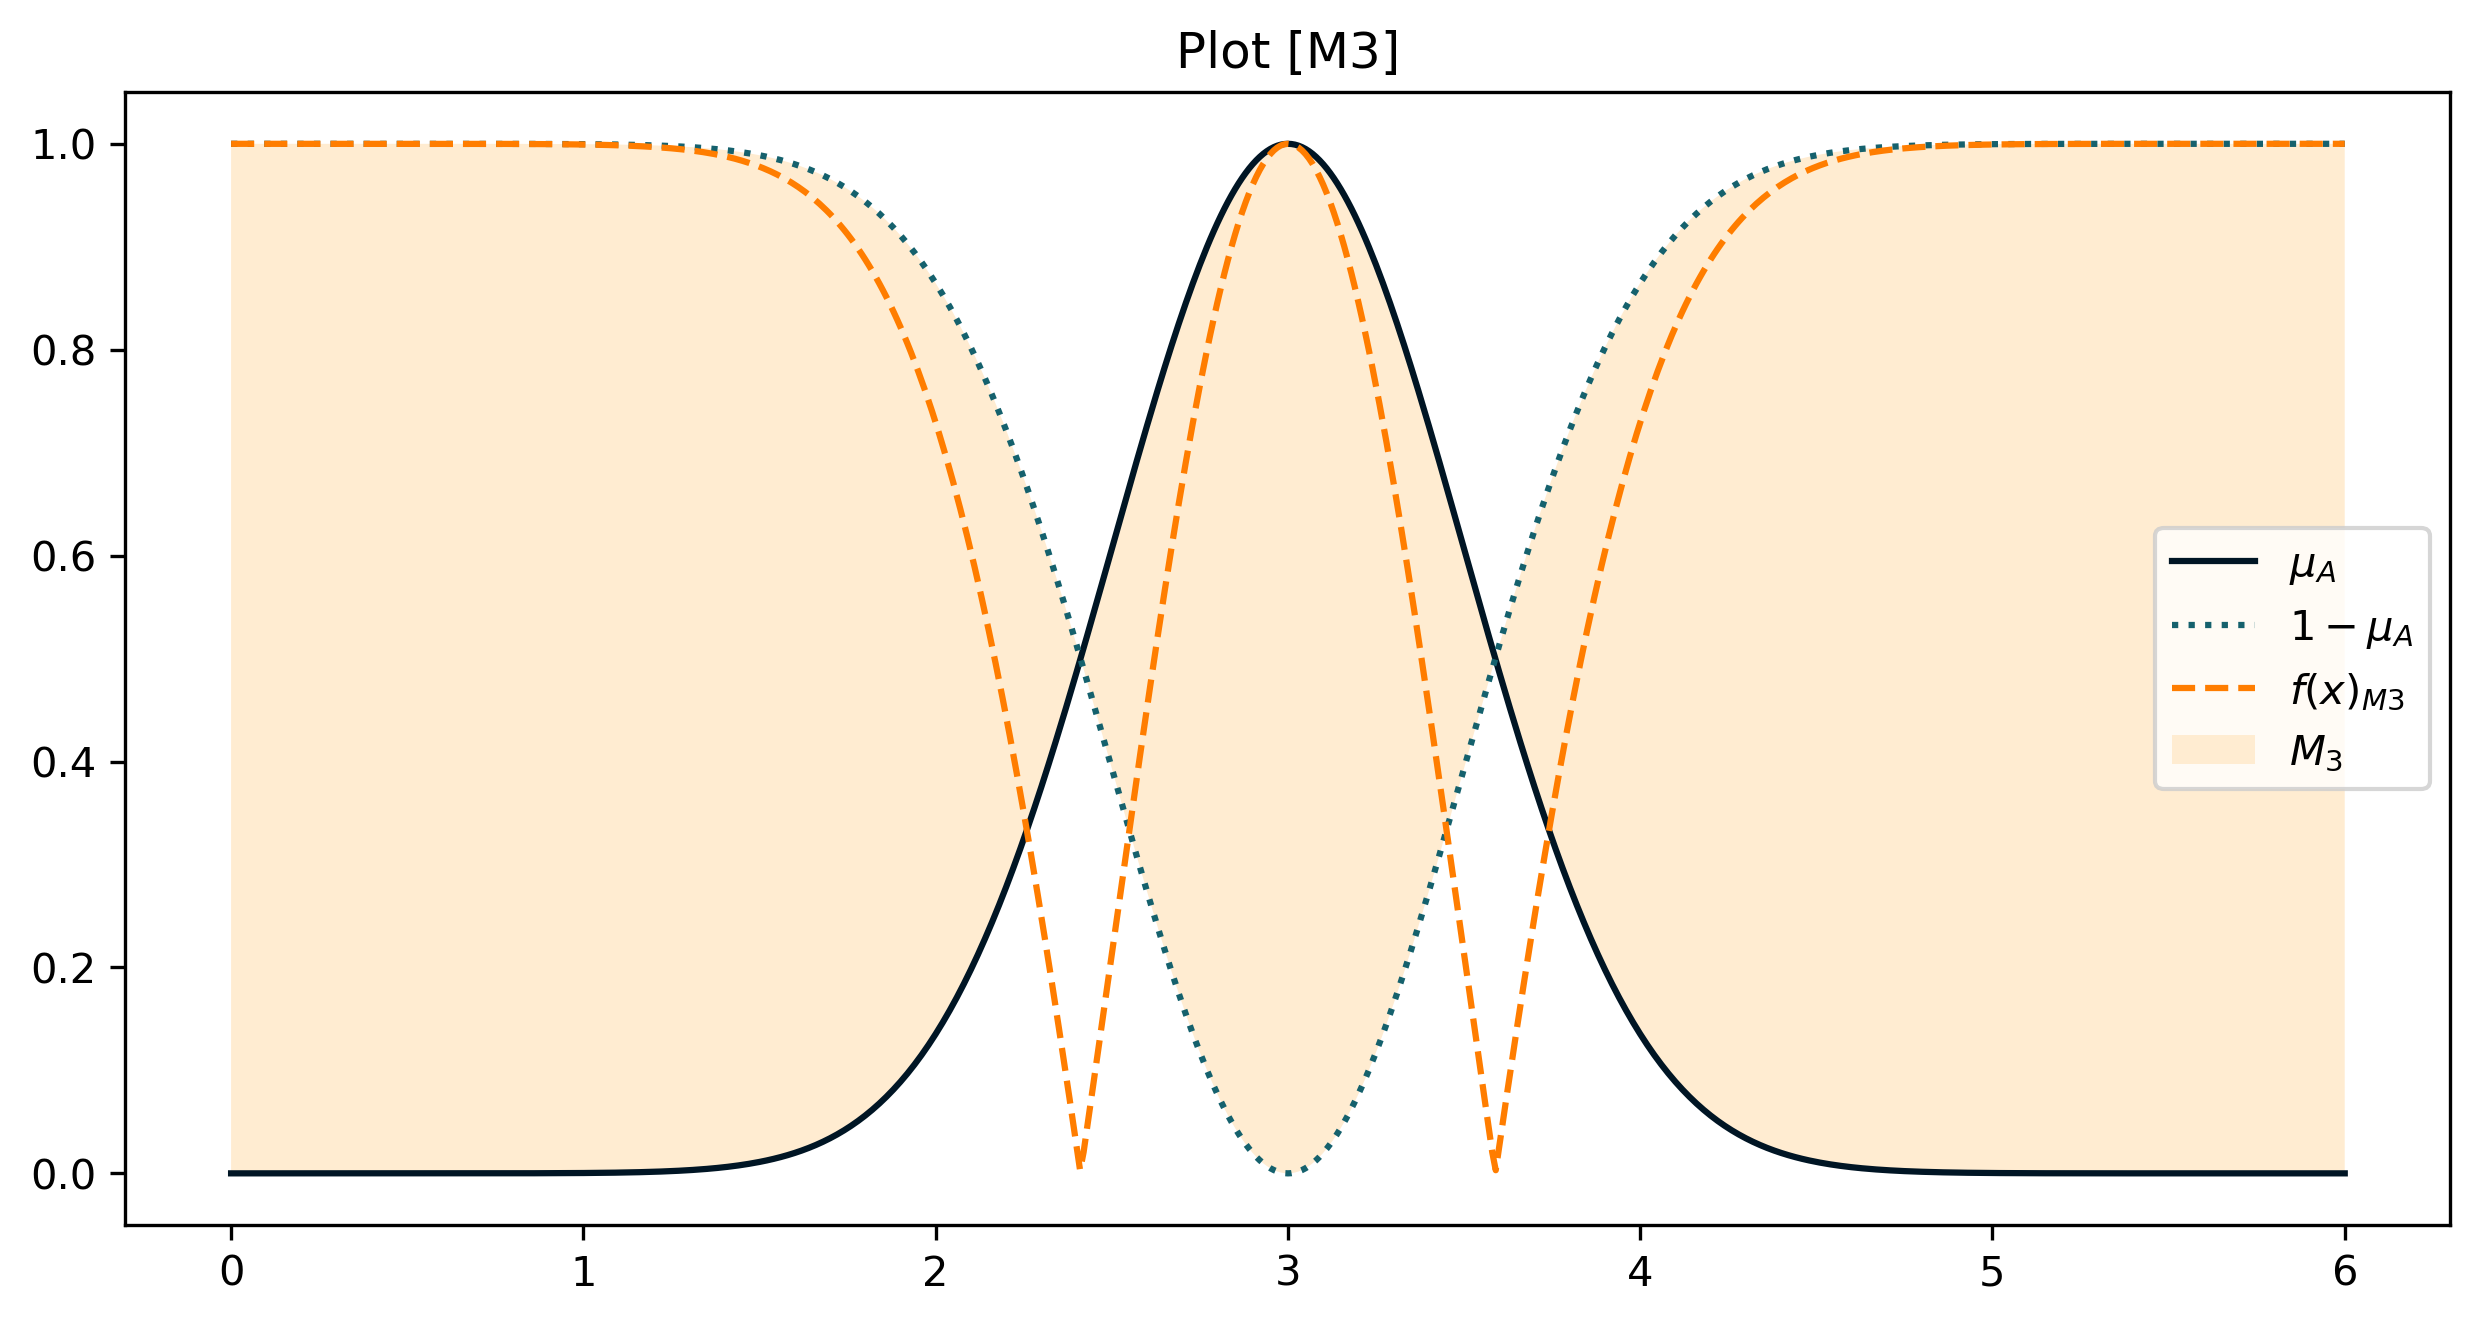
\includegraphics[height=190px]{../src_code/output/P1/plot_M3}}
	\caption{Three Measures of Fuzziness}
	\label{fig:p1}
\end{figure}

\subsection{(i) Relationship between $M_1$, $M_2$, and $M_3$}
The idea is to find the relationship of the function it ($M_i$) integrates from, and then, we can apply the integration to find the final relationship.

Let's define:
\begin{equation}
	 M_1 = \int_S f_{M_1}(x) dx, \quad M_2 = \int_S f_{M_2}(x) dx, \quad M_3 = \int_S f_{M_3}(x) dx \label{eqn:p1:Mi}
\end{equation}

Hence, we may define following functions ($f_{M_1}(x)$, $f_{M_2}(x)$, and $f_{M_3}(x)$):
\begin{align}
	f_{M_1}(x) & = \begin{cases}
		\mu_A(x) & \ifcond \mu_A(x) \leq 0.5 \\
		1-\mu_A(x) & \otherwise
	\end{cases}\\
	f_{M_2}(x) & = |\mu_A(x) - \mu_{A_{1/2}}(x)| \\
	f_{M_2}(x) & = |\mu_A(x) - \mu_{\bar A}(x)| \\
\end{align}

Firstly, let's derive the relationship between $f_{M_1}(x)$ and $f_{M_2}(x)$:
\begin{align}
	f_{M_2}(x) 	& = |\mu_A(x) - \mu_{A_{1/2}}(x)| \\
				& = \begin{cases}
					\mu_A(x) - 1 &\ifcond \mu_A(x) > \alpha = 0.5 \\
					\mu_A(x) &\otherwise
				\end{cases} \\
				& = \begin{cases}
					\mu_A(x) & \ifcond \mu_A(x) \leq 0.5 \\
					1-\mu_A(x) & \otherwise
				\end{cases} \\
				& \equiv f_{M_1}(x) \label{eqn:p1:m2=m1}
\end{align}

Similarly, let's derive the relationship between $f_{M_1}(x)$ and $f_{M_3}(x)$:
\begin{align}
	\because \quad f_{M_3}(x) 	& = |\mu_A(x) - \mu_{\bar A}(x)| \\
				& = |2\mu_A(x) - 1| \\
				& = \begin{cases}
					2\mu_A(x) - 1 &\ifcond (2\mu_A(x) - 1) > 0 \\
					1 - 2\mu_A(x) &\otherwise
				\end{cases} \\
				& = \begin{cases}
					2\mu_A(x) - 1 &\ifcond \mu_A(x) > 0.5 \\
					1 - 2\mu_A(x) &\otherwise
				\end{cases} \\
	1 - f_{M_3}(x) & = \begin{cases}
					2 - 2\mu_A(x) &\ifcond \mu_A(x) > 0.5 \\
					2\mu_A(x) &\otherwise
				\end{cases} \\
	\frac12(1 - f_{M_3}(x)) & = \begin{cases}
					1 - 1\mu_A(x) &\ifcond \mu_A(x) > 0.5 \\
					1\mu_A(x) &\otherwise
				\end{cases} \\
	\frac12(1 - f_{M_3}(x)) &= \begin{cases}
					\mu_A(x) & \ifcond \mu_A(x) \leq 0.5 \\
					1-\mu_A(x) & \otherwise
				\end{cases} \\
				& \equiv f_{M_1}(x) \\
	\therefore \quad f_{M_1}(x) &= \frac12(1 - f_{M_3}(x)) \label{eqn:p1:m3=m1}
\end{align} 

From \Cref{eqn:p1:m2=m1} and \Cref{eqn:p1:m3=m1} we can conclude the following relationships:
\begin{align}
	f_{M_1}(x) = f_{M_2}(x) = \frac12 (1 - f_{M_3}(x))
\end{align}

Finally, based on \Cref{eqn:p1:Mi}, we can derive the final integral relationship between $M_1$, $M_2$, and $M_3$:
\begin{align}
	M_1 = M_2 = \frac12 (1 - M_3)
\end{align}

\subsection{(ii) Comments:}
% Indicate how these measures can be used to represent the degree of fuzziness of a membership function.
%A measure of fuzziness of a fuzzy set $A$ in the universe $X$ defines the closeness of its membership function $\mu_A$ to the \red{most fuzzy grade (0.5)} (cross-over point).
\begin{itemize}
	\item If the membership grade of an element is close to unity, the element is almost definitely a member of set. In contrast, if the membership grade is close to zero, the element is nearly outside the set. Hence, a membership grade of $\mu_A(x)=0.5$ would be the most fuzzy point of an element $x$ in a set $A$, since it has 50-50 chances without preference. As a result, to measure the degree of fuzziness of a membership function, it is simple to integrate or compute the area between the function and $\mu_A(x)=0.5$. 
	\item $M_1$ is the closeness of its membership function $\mu_A$ to the \red{most fuzzy grade (0.5)} as shown in \Cref{fig:p1:M1}, hence, the larger the value, the more fuzzy it is.
	\item $M_2$ is the distance from 1/2 cut line, which measures the distance of membership function from 1/2 cut as seen in \Cref{fig:p1:M2}. Similarly, the larger it is, the fuzzier it becomes.
	\item $M_3$ is the inverse distance from its complement $\mu_{\bar A}$, which computes the distance between the membership function $\mu_A(x)$ and its complement $\mu_{\bar A}(x)$ as highlighted in \Cref{fig:p1:M3}. Hence, in contrast, the larger it is, the less fuzzy it is.
\end{itemize}


%%%%%%%%%%%%%%%%
%%%%% Ex 2 %%%%%
%%%%%%%%%%%%%%%%
\clearpage
\section{Problem 2 (20 marks): Higher Dimension Projection}
\subsection{(a) Total number of Projections:}
\begin{itemize}
	\item Projecting from $n$D to a lower dimension $(n-1)$D requires $n$ times of projections (e.g.: $3D\rightarrow2D: \,k=3$).
	\item Projecting from $n$D to a lower dimension $(n-2)$D requires $n(n-1)$ times of projections (e.g.: $3D\rightarrow1D: \,k=6$).
	\item By induction, we can derive number of projections from $n$D to $(n-r)$D:
	\begin{equation}
		k = n(n-1)\dots(n-(r-1)) = \prod_{j=0}^{r-1} (n - j)
	\end{equation}
	\item But, in fact, there are repetition due to different orders, hence, number of unique projects:
	\begin{align}
		k_{unique}(r=n-m | n\rightarrow m) &= \frac{n}{1} \times \frac{n-1}{2} \times \frac{n-2}{3} \times \frac{n - (r-1)}{r!}\\ 
			& =\frac{n\times (n-1) \times \dots(n-(r-2)) \times \dots(n-(r-1))}{1\times 2\times \dots \times (r-1) \times r} \\
			& = \frac{ \prod_{j=0}^{r-1} (n - j) }{r!} \\
			& \equiv  \prod_{j=0}^{r-1} \frac{(n - j)}{ (1 + j) }
	\end{align}
	(For example: $3D\rightarrow 1D: k = \frac{n(n-1)}{2!} = 3$, with $r=2, n=3$, specifically: unique projection to set $\{X, Y, Z\}$)
	\item As a result, the total number of distinct projection is:
	\begin{align}
		K_{total, unique}(n) &= \sum_{m=1}^{n-1} k_{unique}(r=n-m | n\rightarrow m) \\
		&= \sum_{r=1}^{n-1}  \prod_{j=0}^{r-1} \frac{(n - j)}{ (1 + j) } \\
		&\equiv n + \frac{n(n-1)}{2!} + \frac{n(n-1)(n-2)}{3!} + \dots + \frac{n(n-1)\times\dots\times2}{(n-1)!}
	\end{align}
	(For example: $K(3) = k(3\rightarrow2) + k(3\rightarrow1) = 3 + \frac{3(3-1)}{2!} = 3 + 3 = 6$ unique projections)
\end{itemize}

\subsection{(b) Numerical Examples:}
For simplicity, we will use maximum element-wise operation:
\begin{align}
	\Proj{x_i,y_j,z_k \rightarrow x_i,y_j} R(x_i,y_j,z_k) & = \max_{z_k} R(x_i,y_j,z_k) = 
	\begin{bmatrix} 0.6 & 0.5 & 0.3 \\ 0.4 & 1.0 & 0.6 \\ 0.2 & 0.6 & 0.8 \end{bmatrix} \\
	\Proj{x_i,y_j,z_k \rightarrow y_j,z_k} R(x_i,y_j,z_k) & = \max_{x_i} R(x_i,y_j,z_k) = 
	\begin{bmatrix} 0.5 & 0.8 & 0.6 \\ 0.6 & 1.0 & 0.8 \\ 0.4 & 0.7 & 0.5 \end{bmatrix} \\
	\Proj{x_i,y_j,z_k \rightarrow z_k,x_i} R(x_i,y_j,z_k) & = \max_{y_j} R(x_i,y_j,z_k) = 
	\begin{bmatrix} 0.5 & 0.6 & 0.4 \\ 0.8 & 1.0 & 0.7 \\ 0.6 & 0.8 & 0.5 \end{bmatrix} \\
	\Proj{x_i,y_j,z_k \rightarrow x_i} R(x_i,y_j,z_k) & = \max_{x_i} \Proj{x_i,y_j,z_k \rightarrow x_i,y_j} R(x_i,y_j,z_k) = 
	\begin{bmatrix} 0.6 \\ 1.0 \\ 0.8 \end{bmatrix} \\
	\Proj{x_i,y_j,z_k \rightarrow y_j} R(x_i,y_j,z_k) & = \max_{y_j} \Proj{x_i,y_j,z_k \rightarrow x_i,y_j} R(x_i,y_j,z_k) = 
	\begin{bmatrix} 0.6 & 1.0 & 0.8 \end{bmatrix} \\
	\Proj{x_i,y_j,z_k \rightarrow z_k} R(x_i,y_j,z_k) & = \max_{z_k} \Proj{x_i,y_j,z_k \rightarrow y_j,z_k} R(x_i,y_j,z_k) = 
	\begin{bmatrix} 0.8 \\ 1.0 \\ 0.7 \end{bmatrix} 
\end{align}

Note, there are totally 6 unique projections, 3 from $3D\rightarrow 2D$ and 3 from $3D \rightarrow 1D$. There are two sets of identical projections from $3D \rightarrow 2D$, as listed below:

\begin{align}
	\max_{x_i} \Proj{x_i,y_j,z_k \rightarrow x_i,y_j} & \equiv \max_{x_i} \Proj{x_i,y_j,z_k \rightarrow z_k,x_i} \\
	\max_{y_j} \Proj{x_i,y_j,z_k \rightarrow x_i,y_j} & \equiv \max_{y_j} \Proj{x_i,y_j,z_k \rightarrow y_j,z_k} \\
	\max_{z_k} \Proj{x_i,y_j,z_k \rightarrow z_k,x_i} & \equiv \max_{z_k} \Proj{x_i,y_j,z_k \rightarrow y_j,z_k}
\end{align}

Hence, total $3+3=6$ unique projections.


%%%%%%%%%%%%%%%%
%%%%% Ex 3 %%%%%
%%%%%%%%%%%%%%%%
\clearpage
\section{Problem 3 (20 marks): Fuzzy Logic}
\subsection{(a) Comments on linguistic representations}
\begin{itemize}
	\item The use of translational operator $\mu_F(v-v_0), \text{ with } v_0 > 0$ indicates shifting the centre axis of membership function to right, resulting a much higher standard as the new standard. Consequently, this incorporates "very" to the state, resulting "very fast speed" state from "fast speed".
	\item The square operation of $\mu_F^2 (v)$ behaves like a stretching on the membership function along the $\mu_F$ axis, resulting an amplification on the statement. Hence, the statement of "presumably fast speed" is contradictory to the operator. The operator is stating about "definitely fast speed" instead. To correctly represent "presumably fast speed" with power of 2, the proper operator would be the 2nd order dilation operator: $\mu_F^{1/2}(v)$
\end{itemize}

\subsection{(b) Discrete Example: [See Implementation in \Cref{code:p3}]}
Per discussion, the formal representation would be restated here:
\begin{itemize}
	\item \makebox[5cm]{"very fast speed":\hfill} $\mu_F(v)^{very} = \mu_F(v-v_0), \text{ with } v_0 > 0$ 
	\item \makebox[5cm]{"persumably fast speed":\hfill} $\mu_F(v)^{persumably} = \mu_F^{1/2}(v)$
\end{itemize}

For the given discrete universe $V=\{0,10,20,\dots,200\} \unit{rev/s}$ and $v_0 = 50 \unit{rev/s}$ with the Fuzzy Set F in \Cref{eqn:p3:F}, we may display both membership functions in \Cref{fig:p3:result} and \Cref{table:p3:result} below.
\begin{equation}
		F = \left\{ \frac{0.1}{10}, \frac{0.3}{20}, \frac{0.6}{30}, \frac{0.8}{40}, \frac{1.0}{50}, \frac{0.7}{60}, \frac{0.5}{70}, \frac{0.3}{80}, \frac{0.1}{90}\right\}	 \label{eqn:p3:F}
\end{equation}

\begin{figure}[H]
	\centering
	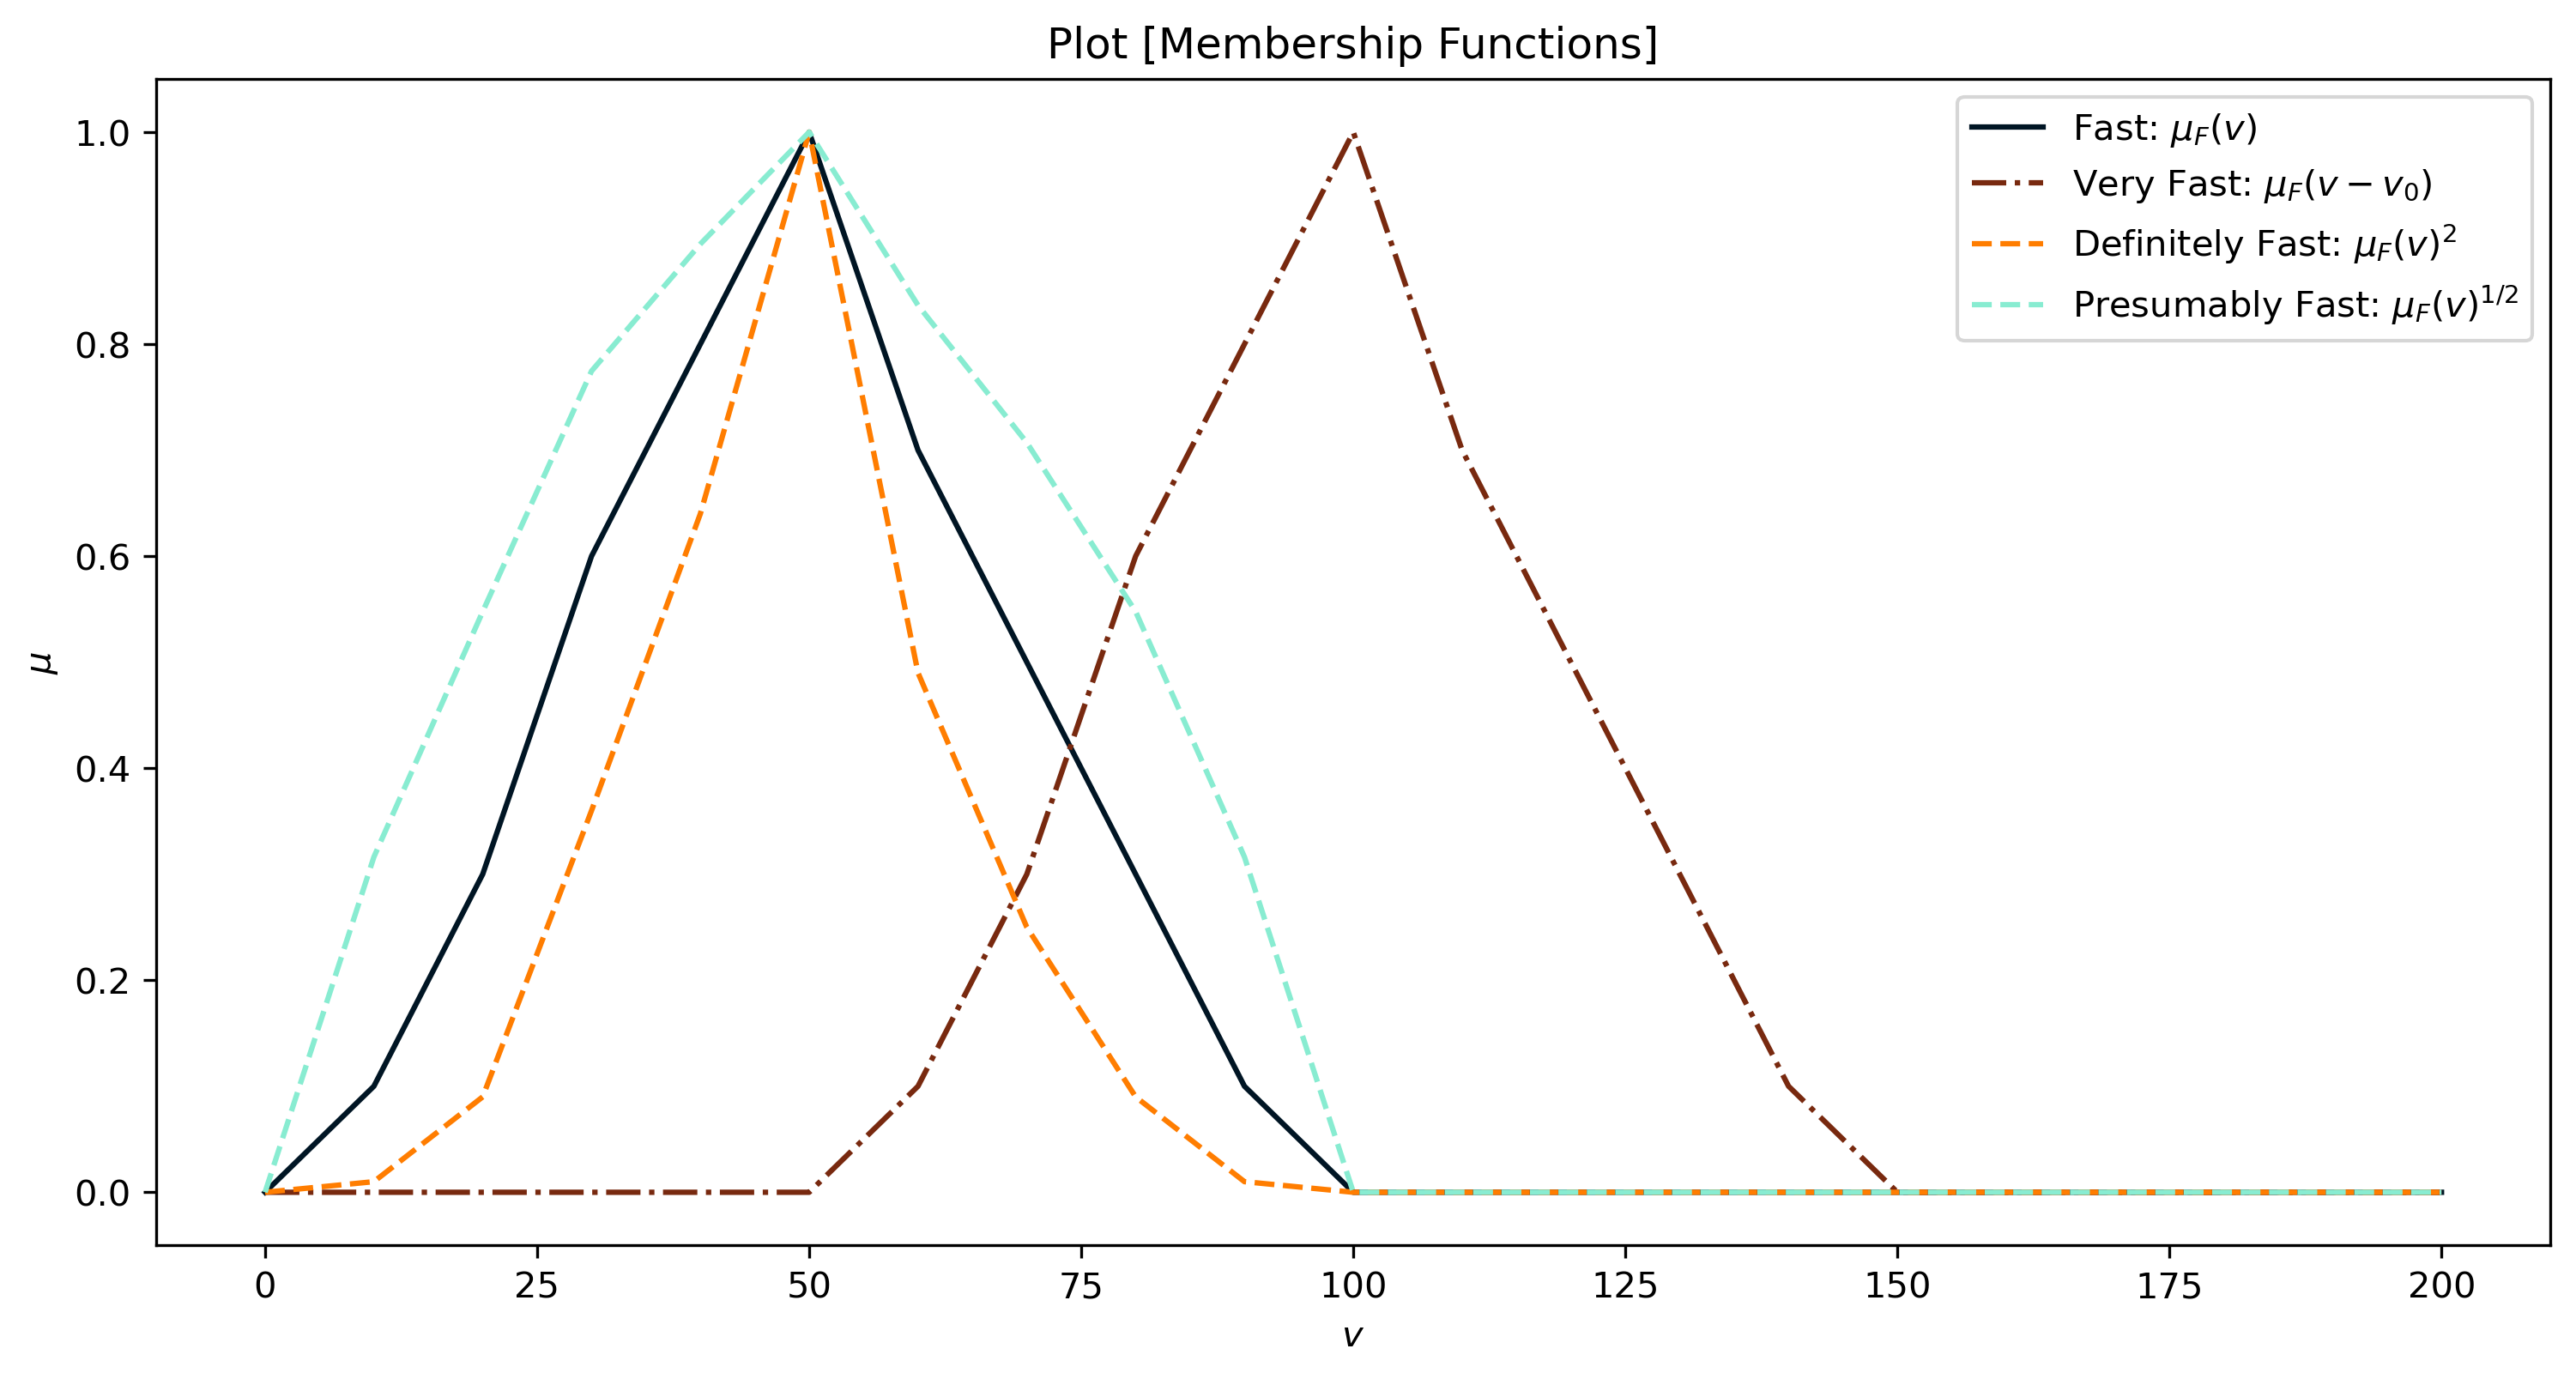
\includegraphics[height=250px]{../src_code/output/P3/plot_Membership Functions}
	\caption{Different membership functions}
	\label{fig:p3:result}
\end{figure}

\begin{table}[H]
  \begin{center}
    \caption{Membership Functions}
    \label{table:p3:result}
		\begin{tabular}{ccccc}
		\hline
		V$\unit{rev/s}$ & Fast & Very Fast & Definitely Fast & Presumably Fast \\
		\hline
		\hline
		0    &   0    &   0   &   0.0   &   0.0   \\
		10   &   0.1  &   0   &   0.01  &   0.32  \\
		20   &   0.3  &   0   &   0.09  &   0.55  \\
		30   &   0.6  &   0   &   0.36  &   0.77  \\
		40   &   0.8  &   0   &   0.64  &   0.89  \\
		50   &   1.0  &   0   &   1.0   &   1.0   \\
		60   &   0.7  &   0.1 &   0.49  &   0.84  \\
		70   &   0.5  &   0.3 &   0.25  &   0.71  \\
		80   &   0.3  &   0.6 &   0.09  &   0.55  \\
		90   &   0.1  &   0.8 &   0.01  &   0.32  \\
		100  &   0    &   1.0 &   0.0   &   0.0   \\
		110  &   0    &   0.7 &   0.0   &   0.0   \\
		120  &   0    &   0.5 &   0.0   &   0.0   \\
		130  &   0    &   0.3 &   0.0   &   0.0   \\
		140  &   0    &   0.1 &   0.0   &   0.0   \\
		150  &   0    &   0   &   0.0   &   0.0   \\
		160  &   0    &   0   &   0.0   &   0.0   \\
		170  &   0    &   0   &   0.0   &   0.0   \\
		180  &   0    &   0   &   0.0   &   0.0   \\
		190  &   0    &   0   &   0.0   &   0.0   \\
		200  &   0    &   0   &   0.0   &   0.0   \\
		\hline
		\end{tabular}
  \end{center}
\end{table}


%%%%%%%%%%%%%%%%
%%%%% Ex 4 %%%%%
%%%%%%%%%%%%%%%%
\clearpage
\section{Problem 4 (5 marks): }
To prove that $\T = \max \{0, x+y - 1\}$ is a \T-norm operator, we need to prove it satisfies the \T-norm properties:
\begin{property-list}
	\item Non-decreasing in each argument. i.e., if $a\leq b$ and $c \leq d$ then $a \T c \leq b\T d$. \label{prop:non-decreasing}
	\item Commutativity: i.e., $a\T b = b\T a$ \label{prop:commmu}
	\item Boundary Conditions: i.e., $a\T 1 = a$ and $a\T 0 = 0$ $\quad \Rightarrow $ take minimum \label{prop:bnd}
	\item Associativity: i.e., $(a\T b)\T c = a\T(b\T c)$ \label{prop:assoc}
\end{property-list}

\begin{proof}[\Cref{prop:non-decreasing}: Non-decreasing]{proof:1}
	\begin{align}
		\text{Let }&  a \leq b, \; c \leq d \\
		a\T c & =  \max \{0, a + c - 1\} \\
		b\T d & =  \max \{0, b + d - 1\} \\
		\therefore \quad & a\T c, \; b\T d\; \geq 0 \\
		\because \quad & a \leq b, \; c \leq d \\
		\therefore \quad & (a + c - 1) \leq (b + d - 1) \\
		\therefore \quad & 0 \leq \max \{0, a + c - 1\} \leq \max \{0, b + d - 1\}\\
		\therefore \quad & 0 \leq a \T c \leq \leq b\T d \\
		\therefore \quad & \text{Satisfy \Cref{prop:non-decreasing}}: a \T c \leq b\T d \quad \ifcond a\leq b \text{ and } c \leq d
	\end{align}d
	\QED
\end{proof}

\begin{proof}[\Cref{prop:commmu}: Commutativity]{proof:2}
	\begin{align}
		\textbf{LHS:}\qquad & = a \T b = \max \{0, a + b - 1\} \\
		\textbf{RHS:}\qquad & = b \T a = \max \{0, b + a - 1\} = \max \{0, a + b - 1\}\\
		\therefore \quad & \textbf{LHS} \equiv \textbf{RHS}\\
		\therefore \quad & \text{Satisfy \Cref{prop:commmu}}: a \T b = b \T a
	\end{align}
	\QED
\end{proof}


\begin{proof}[\Cref{prop:bnd}: Boundary Conditions]{proof:3}
	\begin{align}
		a\T 1  & = \max \{0, a + 1 - 1\} = \max\{0, a\} = a ,\; \forall a\in[0,1]\\
		a\T 0  & = \max \{0, a + 0 - 1\} = \max\{0, a-1 \} = 0,\; \forall a\in[0,1]\\
		\therefore \quad & \text{Satisfy \Cref{prop:bnd}}: a\T 1 = a,\; a\T 0 = 0
	\end{align}
	\QED
\end{proof}

\clearpage
\begin{proof}[\Cref{prop:assoc}: Associativity]{proof:4}
	\begin{align}
		\textbf{LHS:}\qquad & = (a\T b)\T c = \max \left\{ 0, \max \{0, a + b - 1\} + c - 1\right\} \\
							& =  \max \left\{ 0, \max \{c - 1, a + b - 1 + c - 1 \}\right\} \\
						\because \quad & c \in [0,1] \Rightarrow \; (c - 1) \leq 0 \\
							& = \begin{cases}
								0 & \ifcond (a + b + c - 2) \leq 0 \\
								(a + b + c - 2) & \otherwise
							\end{cases} \\
		\textbf{RHS:}\qquad & = a\T(b\T c) = \max \left\{ 0, a + \max \{0, b + c - 1\} - 1\right\} \\
							& =  \max \left\{ 0, \max \{a - 1, a + b + c - 1 - 1\} \right\} \\
						\because \quad & a \in [0,1] \Rightarrow \; (a - 1) \leq 0 \\
							& = \begin{cases}
								0 & \ifcond (a + b + c - 2) \leq 0 \\
								(a + b + c - 2) & \otherwise
							\end{cases} \\
		\therefore \quad & \textbf{LHS} \equiv \textbf{RHS}\\
		\therefore \quad & \text{Satisfy \Cref{prop:assoc}}: (a\T b)\T c = a\T(b\T c)
	\end{align}
	\QED
\end{proof}

Hence, as proved above in \Cref{proof:1}, \Cref{proof:2}, \Cref{proof:3}, and \Cref{proof:4}, it is confirmed that $\T = \max \{0, x+y - 1\}$ is a \T-norm operator.

Now, let's derive for the \T-conorm (aka. \Snorm-norm) from DeMorgan's Law:
\begin{align}
	a\Snorm b 	& = \overline{\bar a \T \bar b} \\
				& = 1 - \left[  \max \{0, (1-a) + (1-b) - 1\}  \right] \\
				& = 1 -\left[  \max \{0, 1 - a - b \}  \right] \\
				& = 1 +\left[  \min \{0, a + b - 1 \}  \right] \\
				& = \min \{1, a + b \} \\
	\therefore \qquad \Snorm & = \min \{1, x + y \}
\end{align}

%%%%%%%%%%%%%%%%
%%%%% Ex 5 %%%%%
%%%%%%%%%%%%%%%%
\clearpage
\section{Problem 5 (10 marks): [See implementation in \Cref{code:p5}]}
As implemented in \Cref{code:p5}, we have plotted the membership function $\mu_A(x) = \exp \{ -\lambda |x-a|^n\}$ below, by varying its parameters.

\paragraph{Varying $a$:}
As we may see from \Cref{fig:p5:a}, the $a$ changes the center of the membership function but it does not affect its shape. As $a$ increases, the membership function translates towards to the right side, this leads towards an amplification of "very" from the fuzzy modifier. Conversely, as $a$ decreases, the membership function translates towards the left side, attenuate the fuzzy state, and the state become "less". The fuzziness remains unchanged $\forall a$.
\begin{figure}[H]
	\centering
	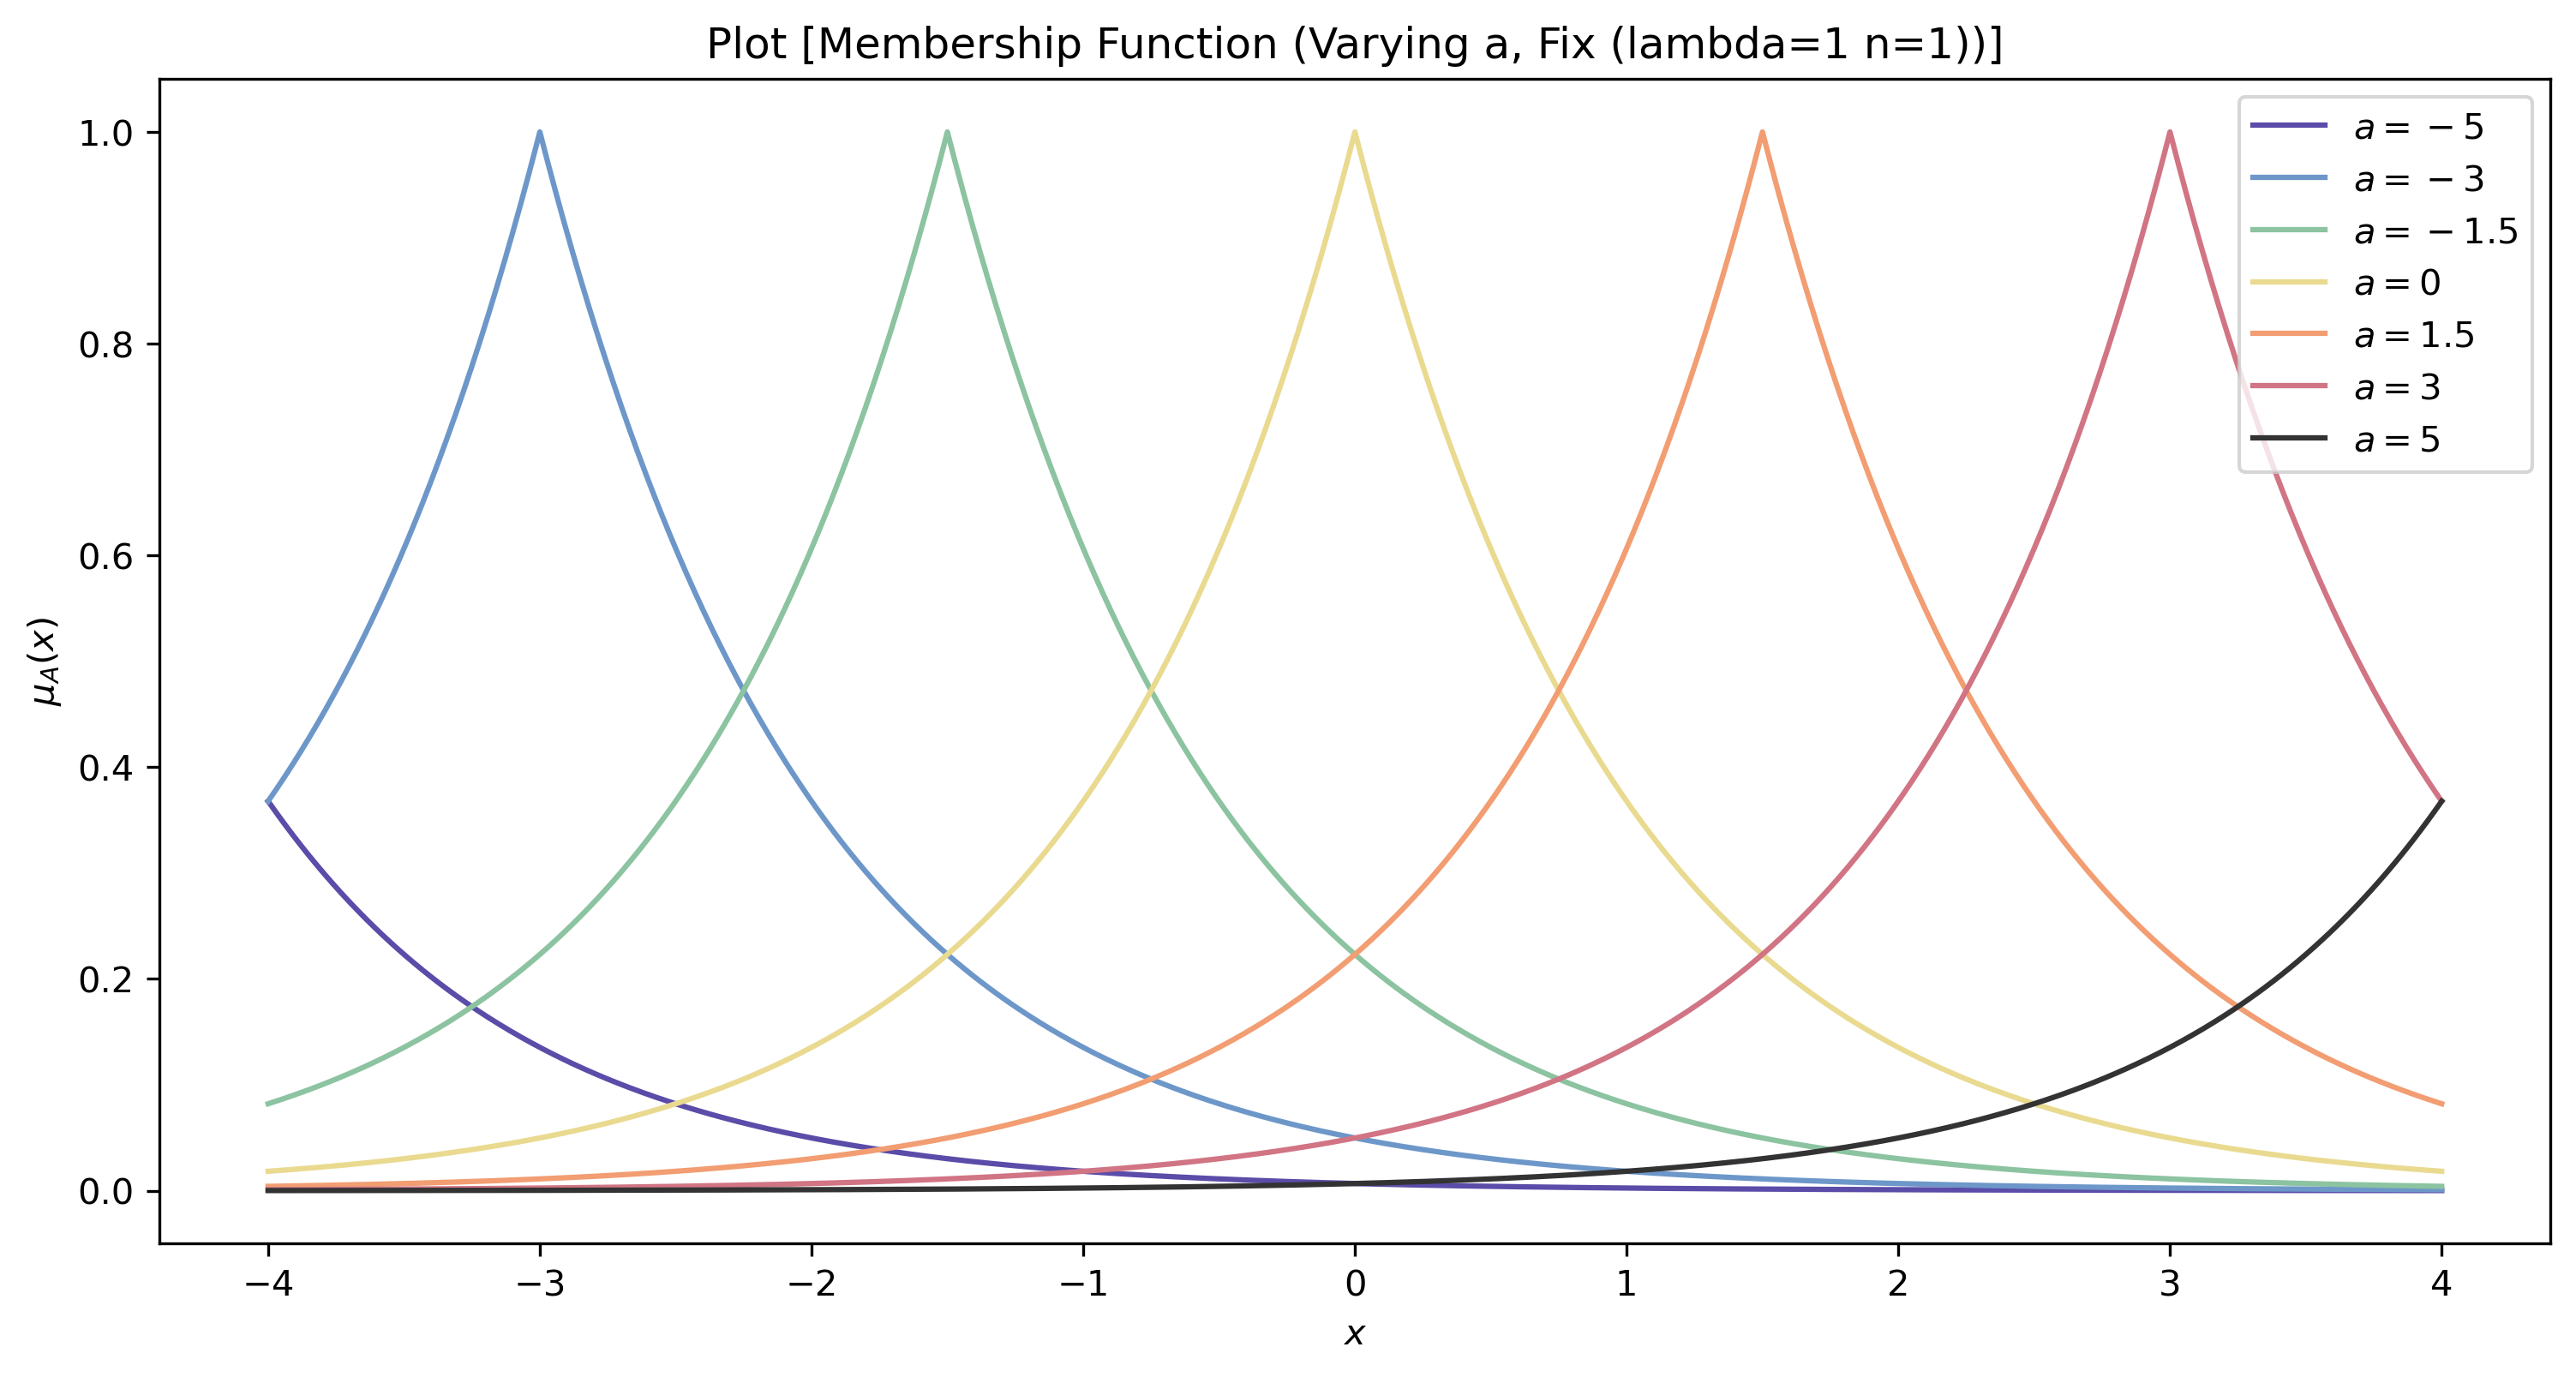
\includegraphics[height=250px]{../src_code/output/P5/plot_Membership Function (Varying a, Fix (lambda=1 n=1))}
	\caption{Varying $a$}
	\label{fig:p5:a}
\end{figure}

\clearpage
\paragraph{Varying $\lambda$:}
As we may see from \Cref{fig:p5:lambda}, the $\lambda$ changes the shape of the membership function. An increasing $\lambda$ leads to a narrower graph, resulting a contraction effect to the fuzzy state. Hence, an increasing $\lambda$ would make the fuzzy state more firm (or less fuzziness). In contrast, when reducing the $\lambda$ towards 0, it makes the fuzzy state more "presumable" and uncertain. At the $\lambda \leq 0$, the whole fuzzy state is completely useless, since $\mu_A(x) = 1 \; \forall x\in \RR$.
\begin{figure}[H]
	\centering
	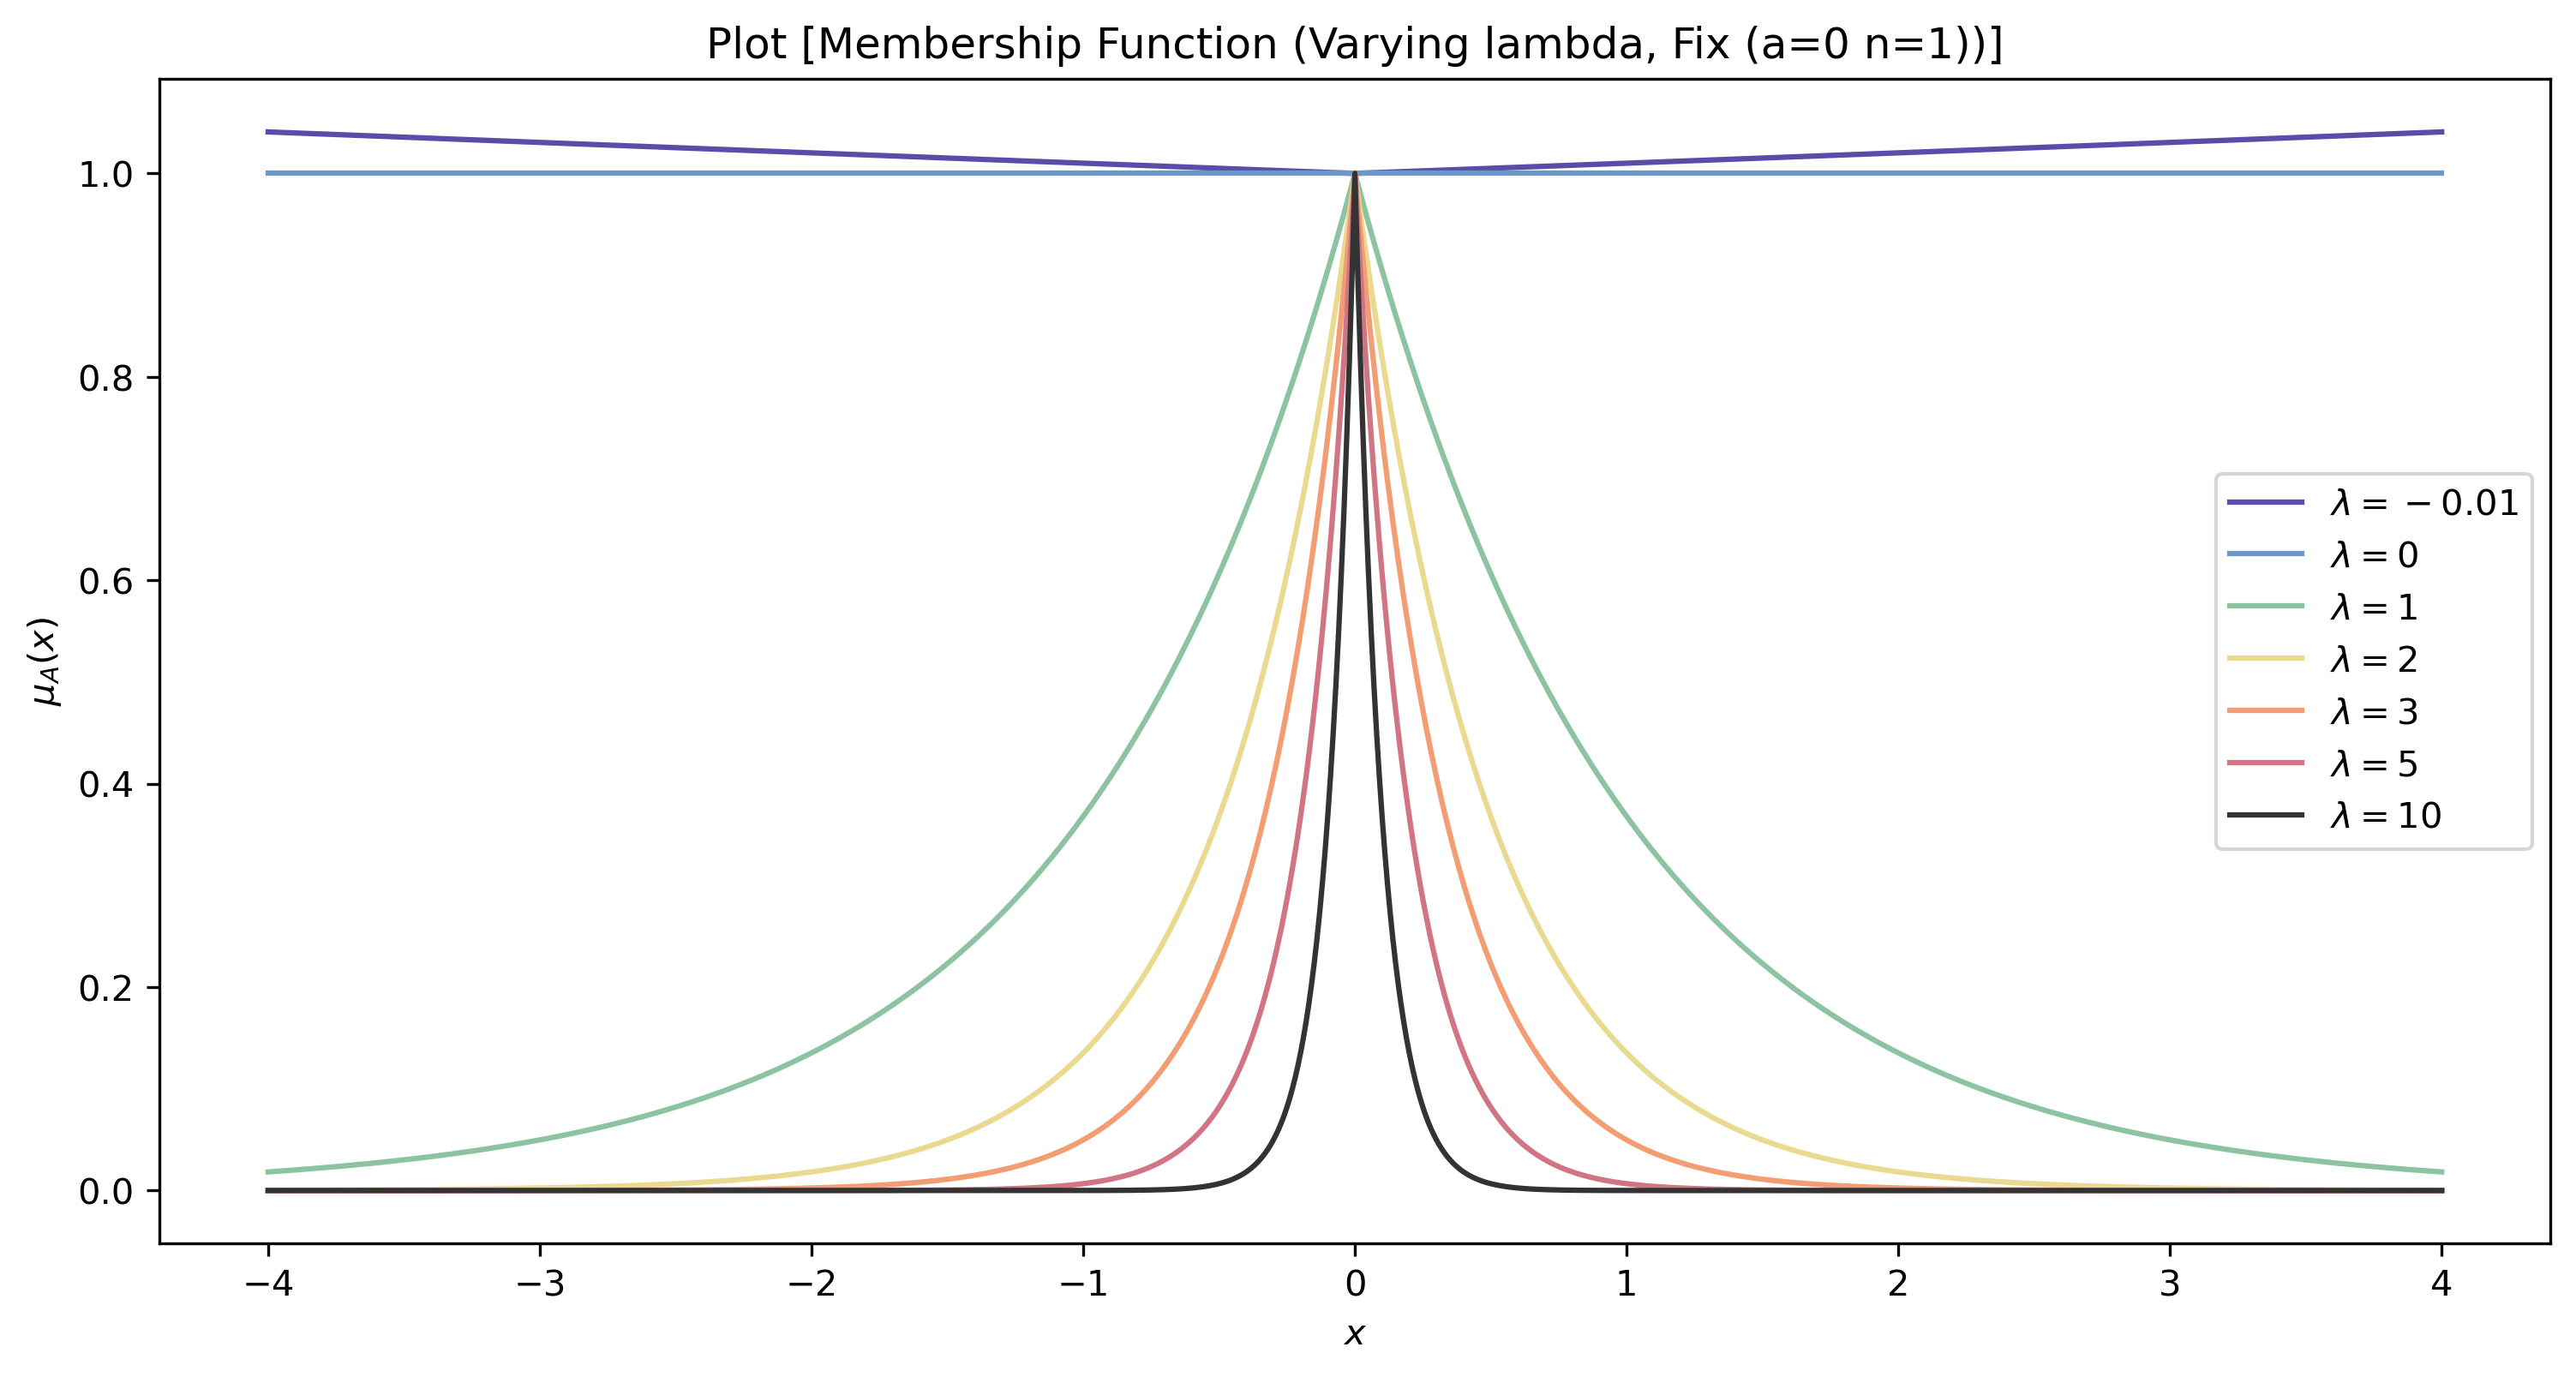
\includegraphics[height=250px]{../src_code/output/P5/plot_Membership Function (Varying lambda, Fix (a=0 n=1))}
	\caption{Varying $\lambda$}
	\label{fig:p5:lambda}
\end{figure}

\clearpage
\paragraph{Varying $n$}
As we may see from \Cref{fig:p5:n}, the $n$ changes the shape of the membership function. When $n > 0$, an increasing $n$ results a sharper pulse curve, and it tends toward to form a shape of a unit pulse as $n\rightarrow \infty$. As a result, an increasing $n$ decreases the fuzziness of the membership function, resulting a much more firm state. In contrast, as the $n$ decreases, the state becomes fuzzier and more uncertain ("somehow"). However, when $n < 0$, the membership function flips, resulting a flipped effects: the smaller $n<0$ is, it becomes less fuzzy, besides the fact that the entire state is flipped. Hence, the smaller $n<0$ is towards $-\infty$, it becomes more "very not".
\begin{figure}[H]
	\centering
	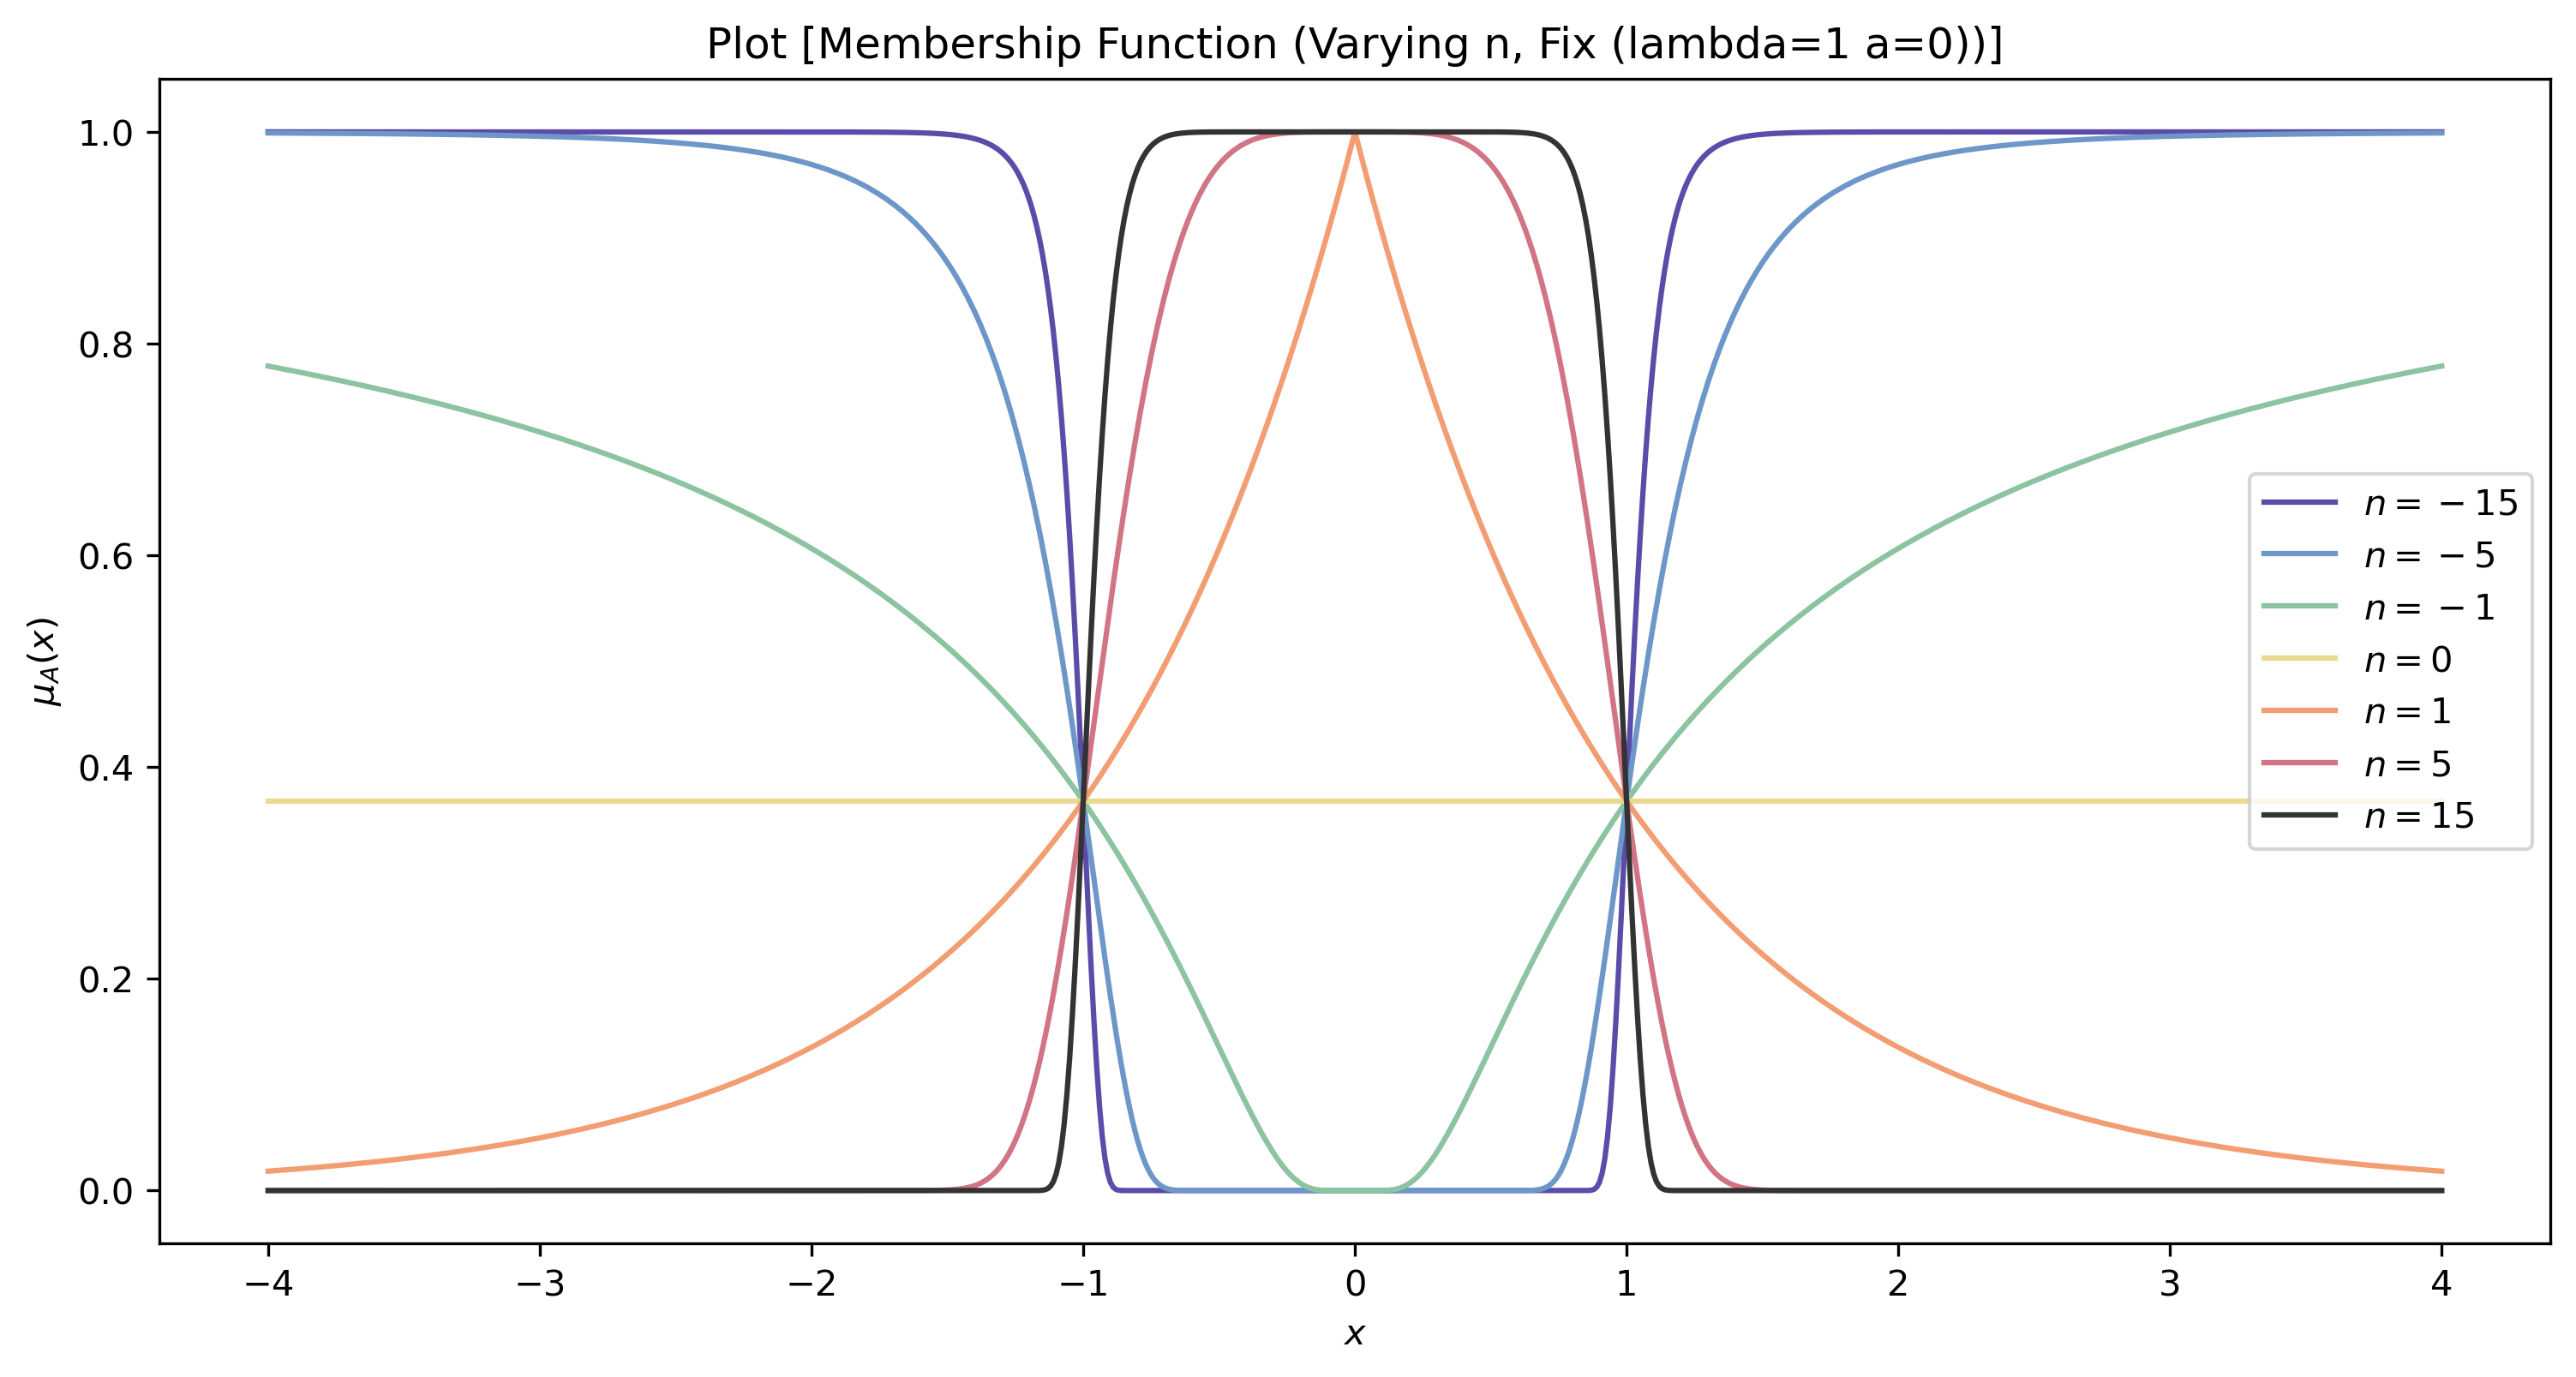
\includegraphics[height=250px]{../src_code/output/P5/plot_Membership Function (Varying n, Fix (lambda=1 a=0))}
	\caption{Varying $n$}
	\label{fig:p5:n}
\end{figure}



%%%%%%%%%%%%%%%%
%%%%% Ex 6 %%%%%
%%%%%%%%%%%%%%%%
\clearpage
\section{Problem 6 (20 marks): [See implementation in \Cref{code:p6}]}
\subsection{(a) Four rules in membership diagram:}
\begin{figure}[H]
	\centering
	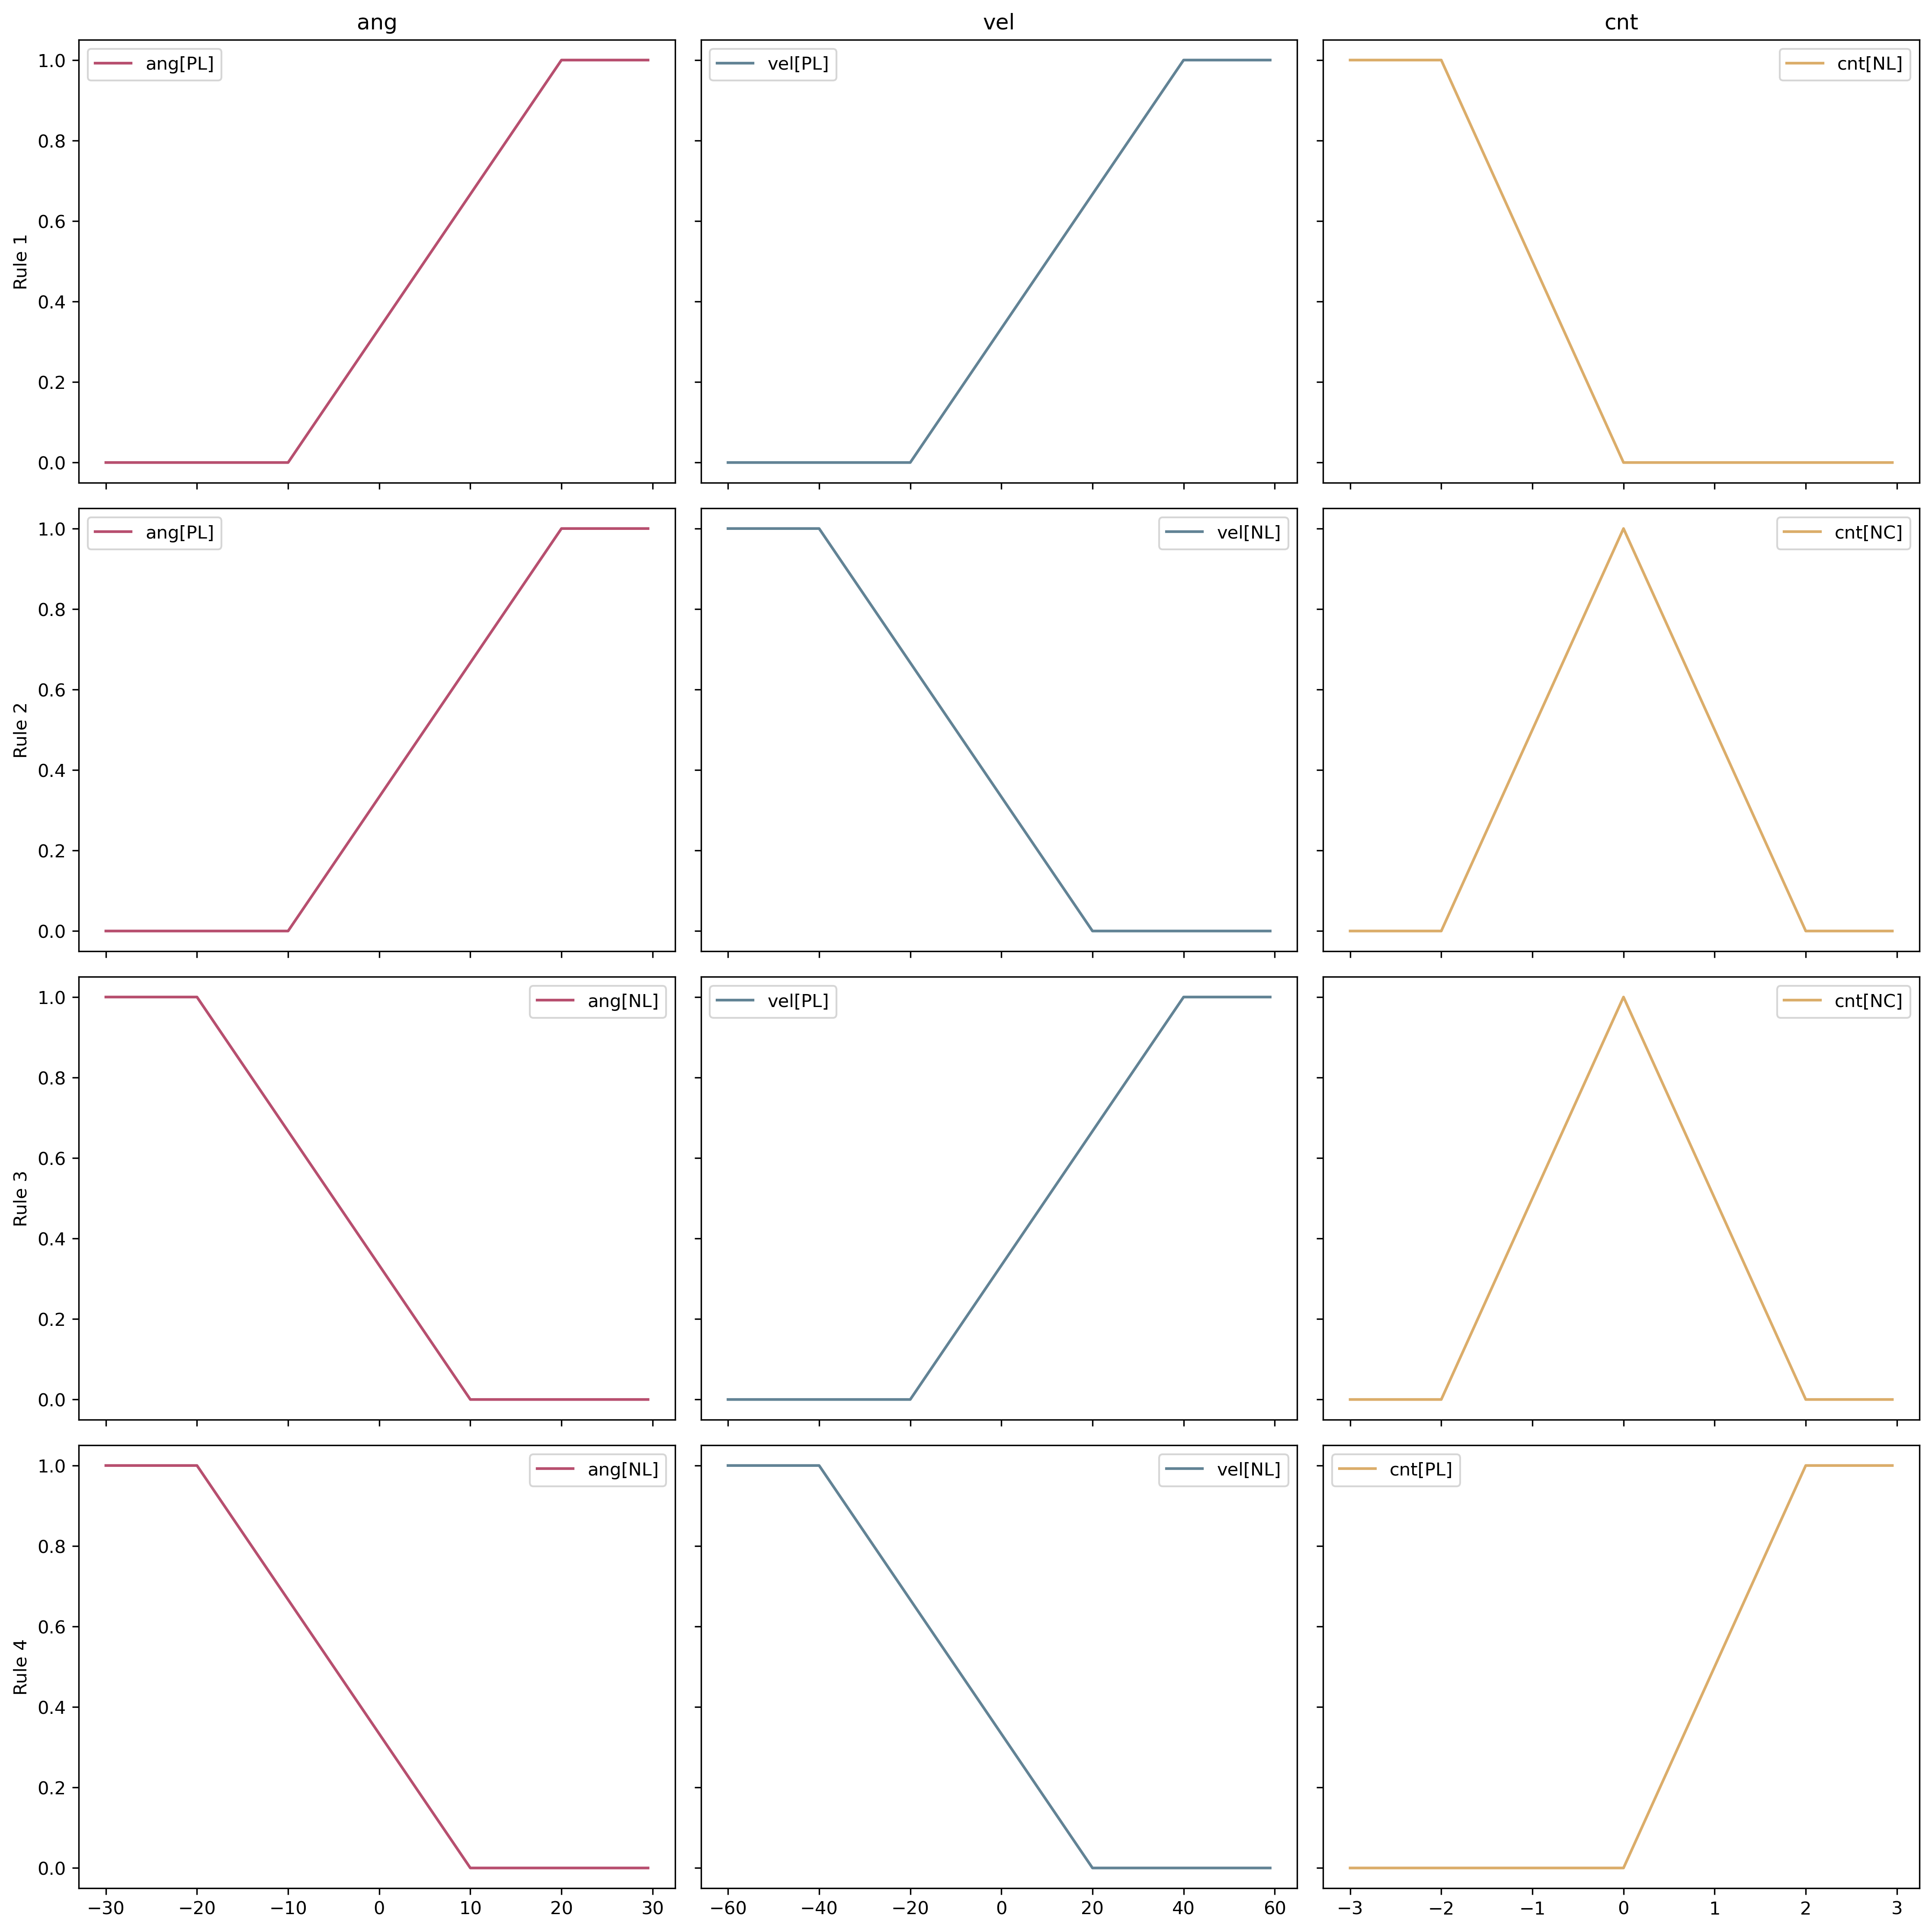
\includegraphics[height=500px]{../src_code/output/P6/plot_Rule-Based Inference}
	\caption{Sketch of the four rules in a membership diagram for the purpose of making control inferences using individual rule-based inference}
	\label{fig:p5:n}
\end{figure}

\subsection{(b) Process Measurements of $ANG = 5^{\circ}$ and $VEL = 15^{\circ}/s$:}
\begin{figure}[H]
	\centering
	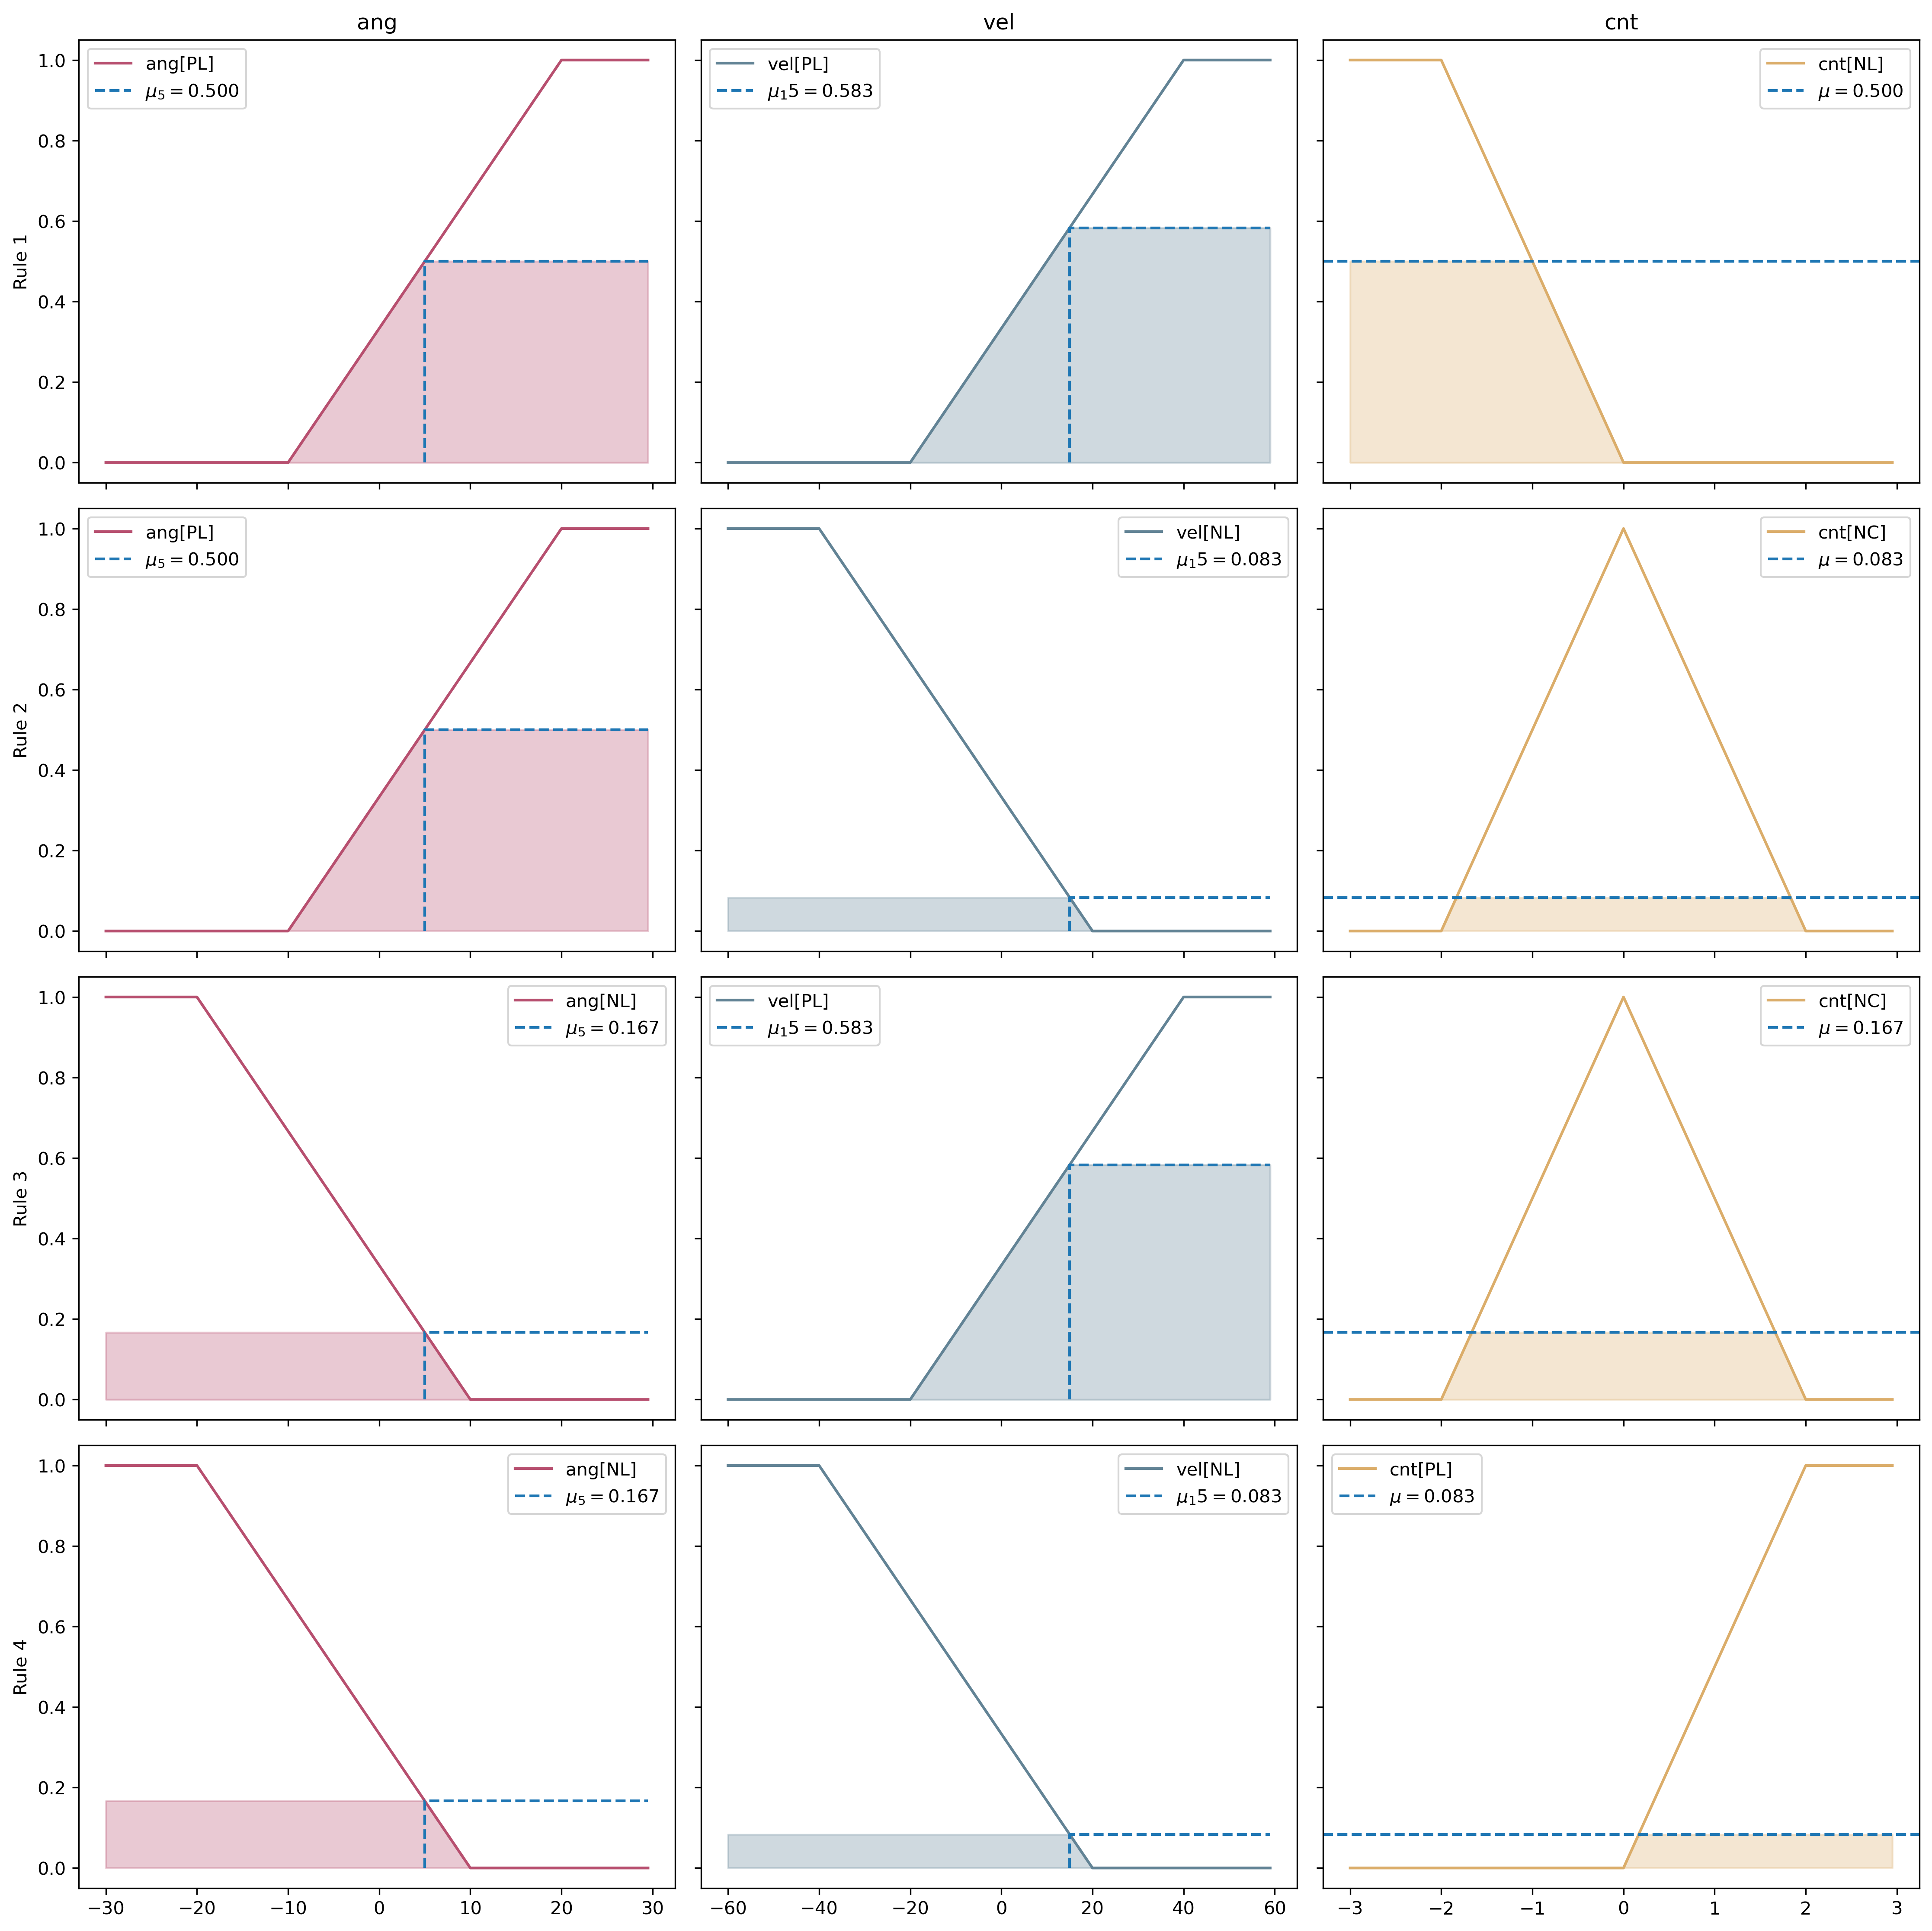
\includegraphics[height=500px]{../src_code/output/P6/plot_Control Inference}
	\caption{Sketch with corresponding control inference}
	\label{fig:p5:n}
\end{figure}

\clearpage
As a result, the final control value was determined to be $-1.02A$ from the final control inference plot shown below:
\begin{figure}[H]
	\centering
	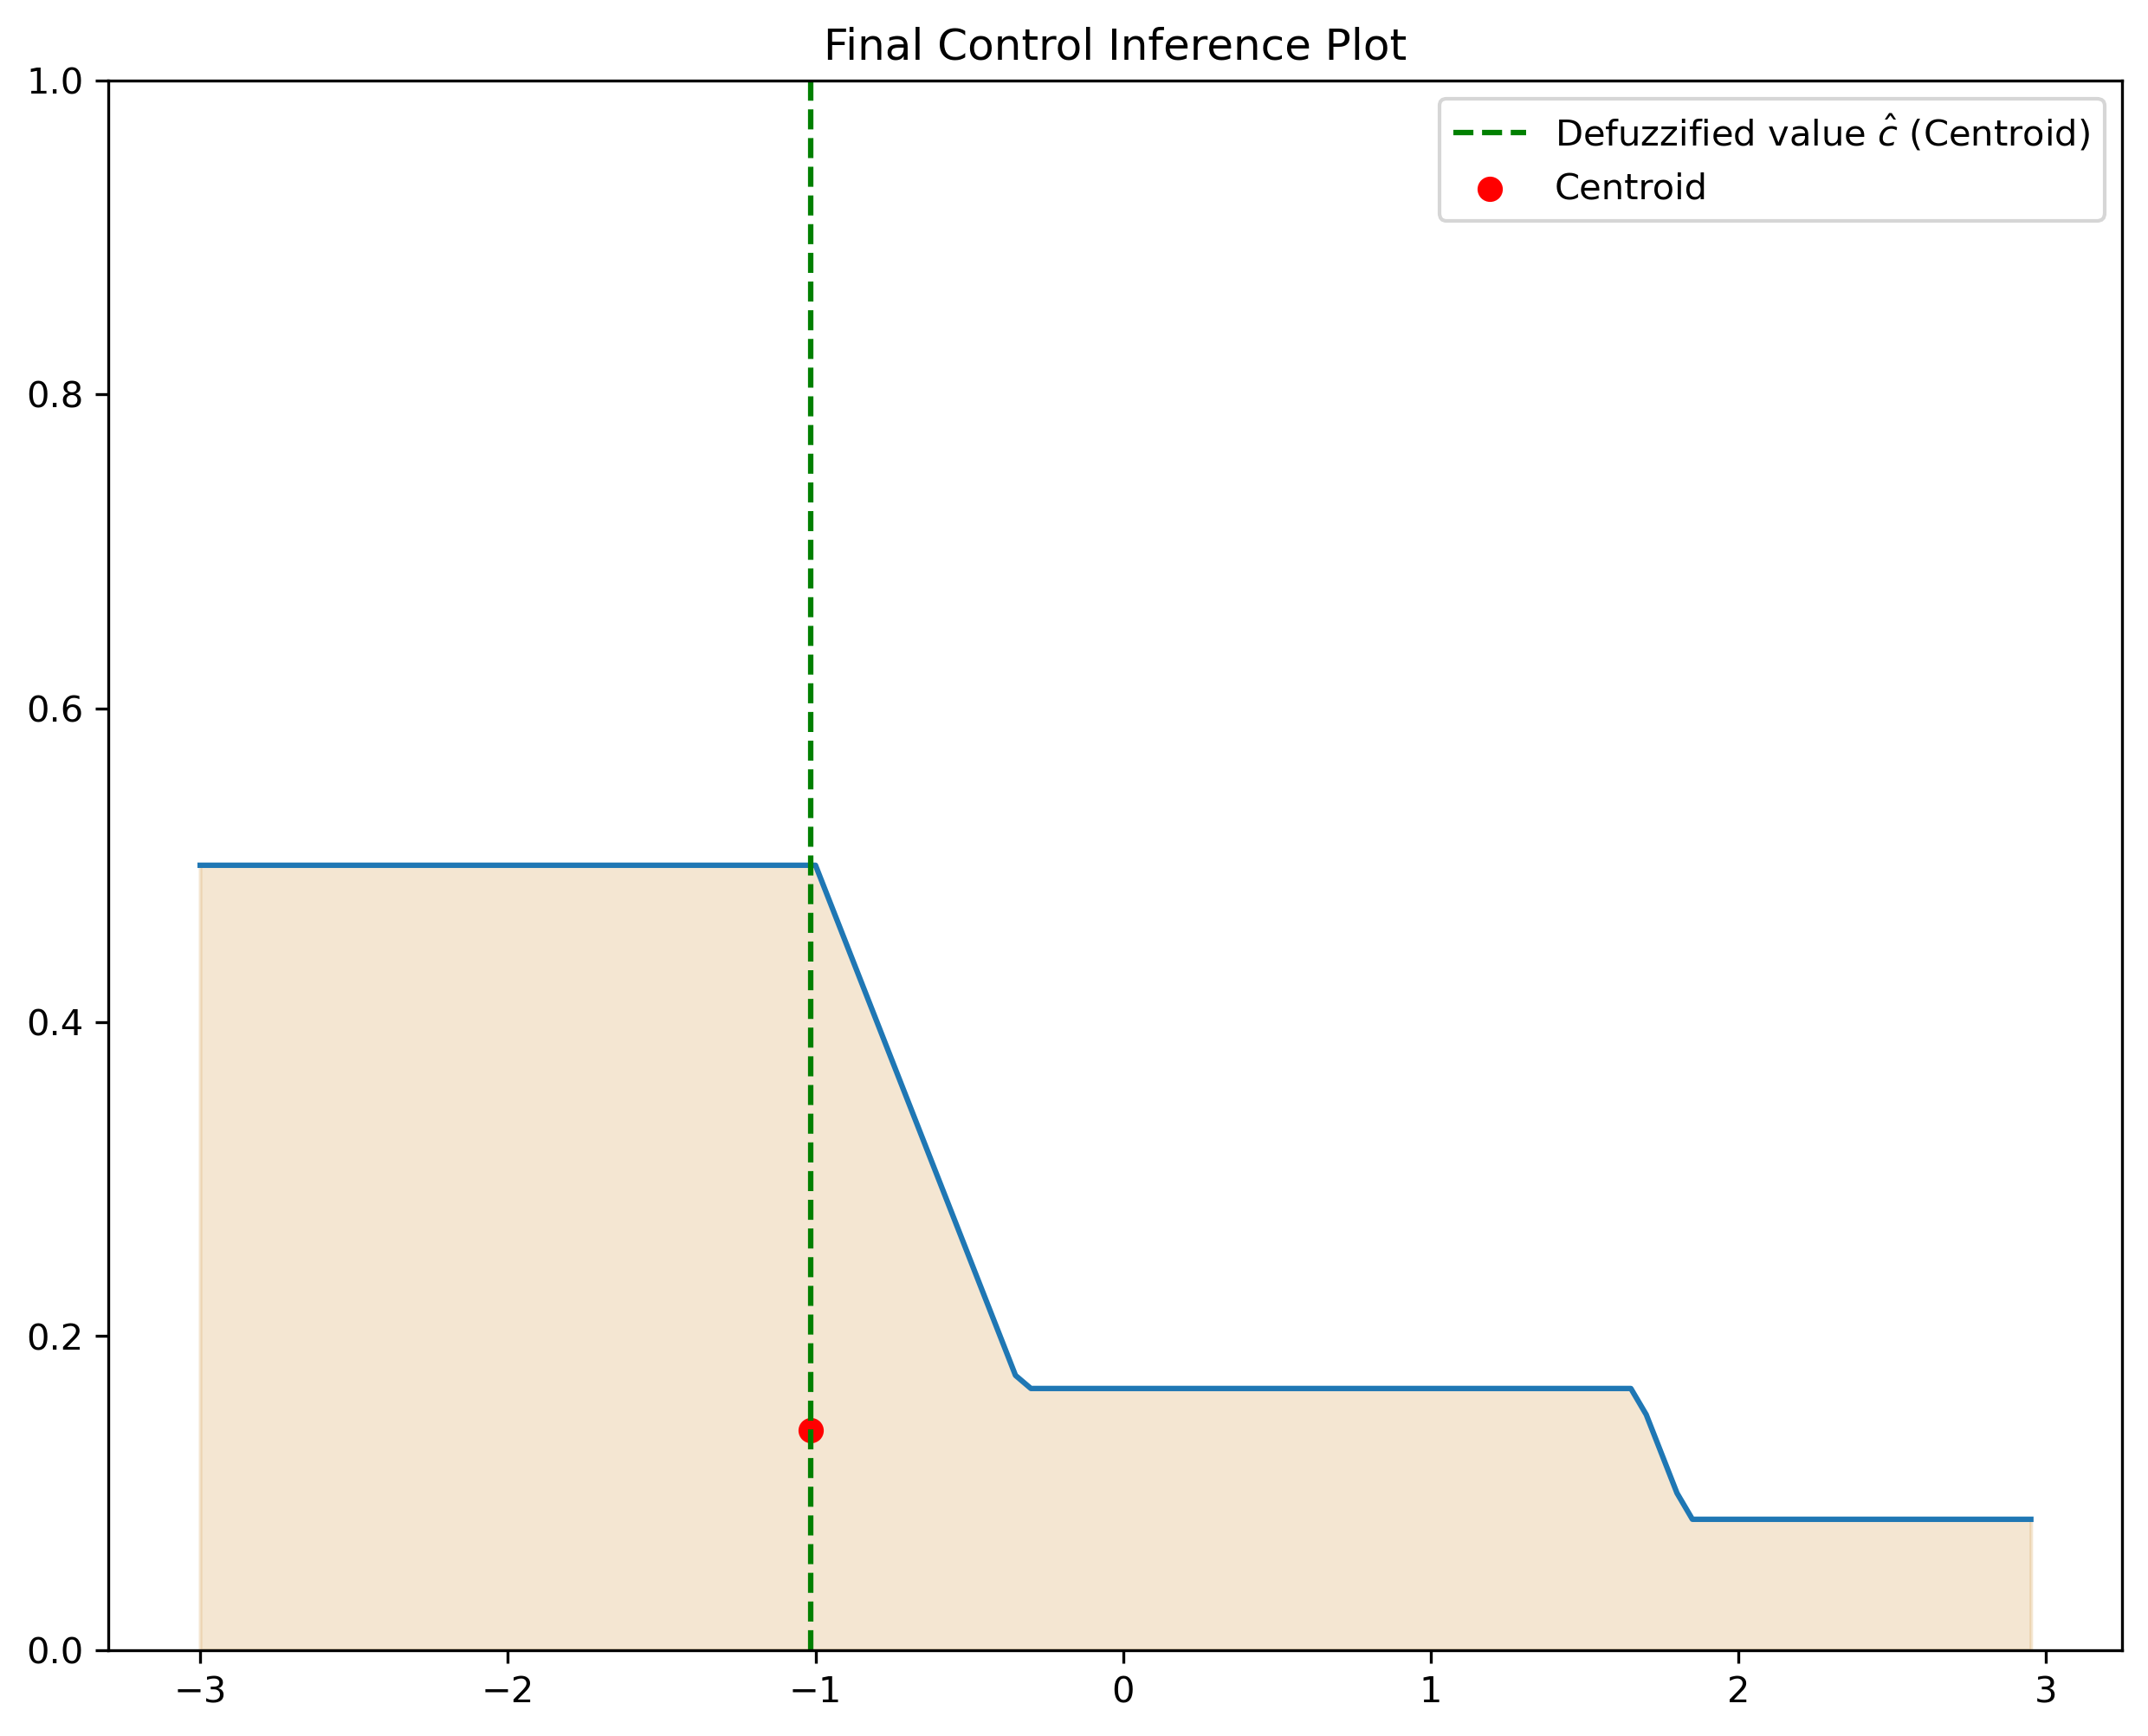
\includegraphics[height=300px]{../src_code/output/P6/plot_final_control_Control Inference}
	\caption{Sketch with corresponding control inference}
	\label{fig:p5:n}
\end{figure}

%%%%%%%%%%%%%%%%%%%%%%%%%%%%%%%%%%%%%%%%%%%%%%%%%%%%%%%%%%%%%%%%%%%%%%%%%%%%%%%%
%% ************************************************************************** %%
%% *                      TODO [Remove For Final Copy!]                     * %%
%% ************************************************************************** %%
%%%%%%%%%%%%%%%%%%%%%%%%%%%%%%%%%%%%%%%%%%%%%%%%%%%%%%%%%%%%%%%%%%%%%%%%%%%%%%%%
%\printlistoftodos

%%%%%%%%%%%%%%%%%%%%%%%%%%%%%%%%%%%%%%%%%%%%%%%%%%%%%%%%%%%%%%%%%%%%%%%%%%%%%%%%
%% ************************************************************************** %%
%% *                                Glossary                                * %%
%% ************************************************************************** %%
%%%%%%%%%%%%%%%%%%%%%%%%%%%%%%%%%%%%%%%%%%%%%%%%%%%%%%%%%%%%%%%%%%%%%%%%%%%%%%%%
%\clearpage
%\printglossaries

%%%%%%%%%%%%%%%%%%%%%%%%%%%%%%%%%%%%%%%%%%%%%%%%%%%%%%%%%%%%%%%%%%%%%%%%%%%%%%%%
%% ************************************************************************** %%
%% *                               References                               * %%
%% ************************************************************************** %%
%%%%%%%%%%%%%%%%%%%%%%%%%%%%%%%%%%%%%%%%%%%%%%%%%%%%%%%%%%%%%%%%%%%%%%%%%%%%%%%%

% \printbibliography[heading=none]

%%%%%%%%%%%%%%%%%%%%%%%%%%%%%%%%%%%%%%%%%%%%%%%%%%%%%%%%%%%%%%%%%%%%%%%%%%%%%%%%
%% ************************************************************************** %%
%% *                               Appendices                               * %%
%% ************************************************************************** %%
%%%%%%%%%%%%%%%%%%%%%%%%%%%%%%%%%%%%%%%%%%%%%%%%%%%%%%%%%%%%%%%%%%%%%%%%%%%%%%%%
% appendices use section and subsection numbering
\newpage
\appendix
\begin{appendices}
% INPUT UR APPENDIX
\section{Problem 1}
\lstinputlisting[language=python, caption=Main Code for P1, label=code:p1]{../src_code/main_a3p1.py}

\section{Problem 3}
\lstinputlisting[language=python, caption=Main Code for P3, label=code:p3]{../src_code/main_a3p3.py}

\section{Problem 5}
\lstinputlisting[language=python, caption=Main Code for P3, label=code:p5]{../src_code/main_a3p5.py}

\section{Problem 6}
\lstinputlisting[language=python, caption=Main Code for P3, label=code:p6]{../src_code/main_a3p6.py}

%\section{Handy Custom Library}
%\lstinputlisting[language=python, caption=My Custom Library, label=code:jx_lib]{../src_code/jx_lib.py}


\end{appendices}

\end{document}


